\subsection{Termalizzazione}

\vspace*{\fill}

\begin{figure}[H]
    \centering
    \begin{minipage}{0.45\textwidth}  
      \centering
      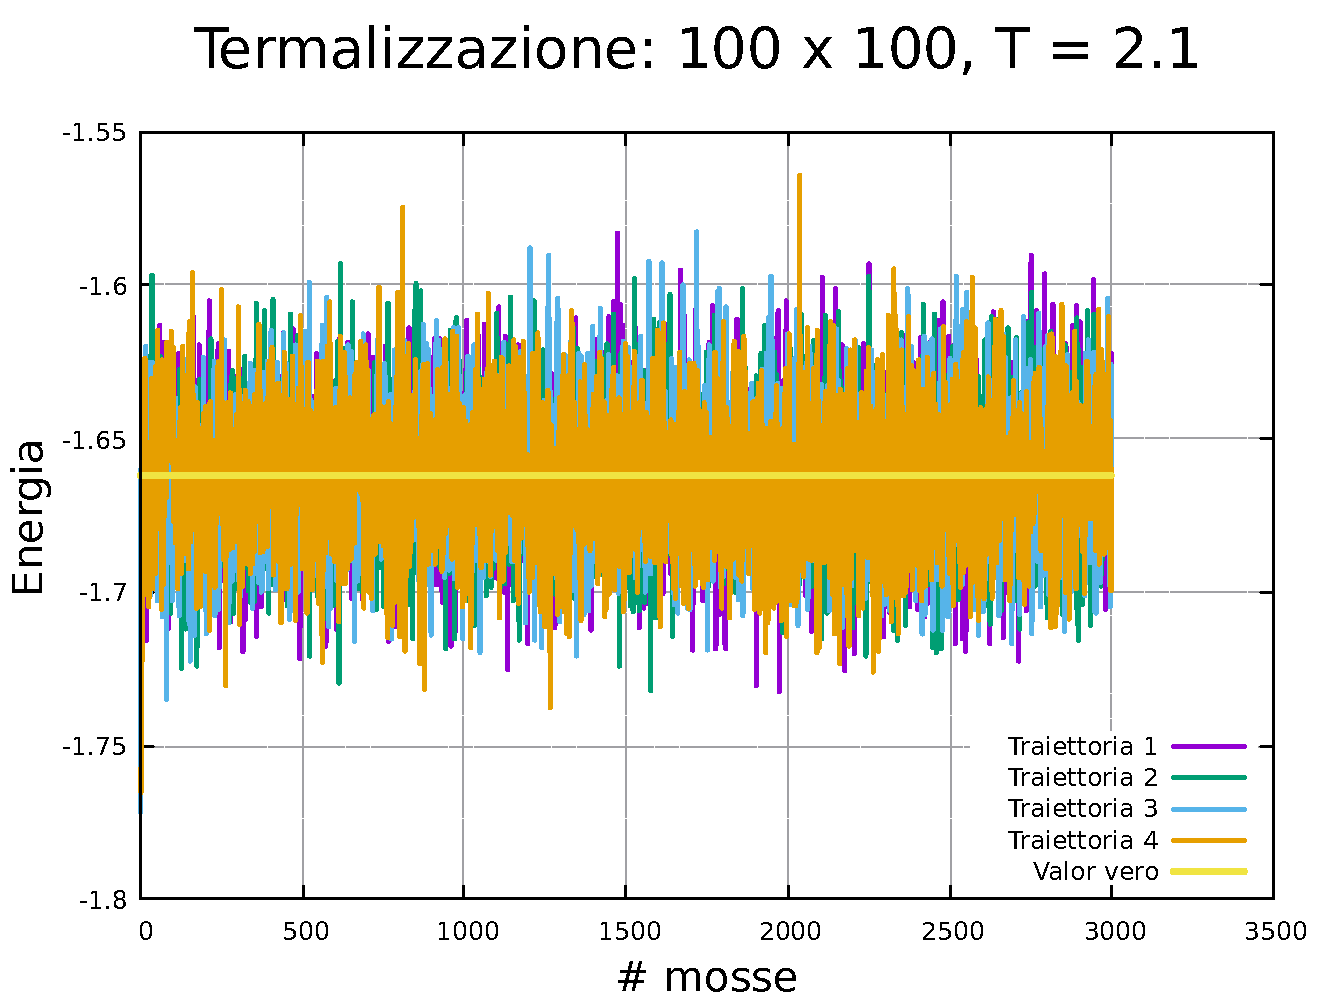
\includegraphics[page=1, width=\textwidth]{Immagini/simIsing2D/wolff/term/term_100_2.1.pdf}
      \caption{$T\,=\,1.0$}
    \end{minipage}\hfill
    \begin{minipage}{0.45\textwidth}  
      \centering
      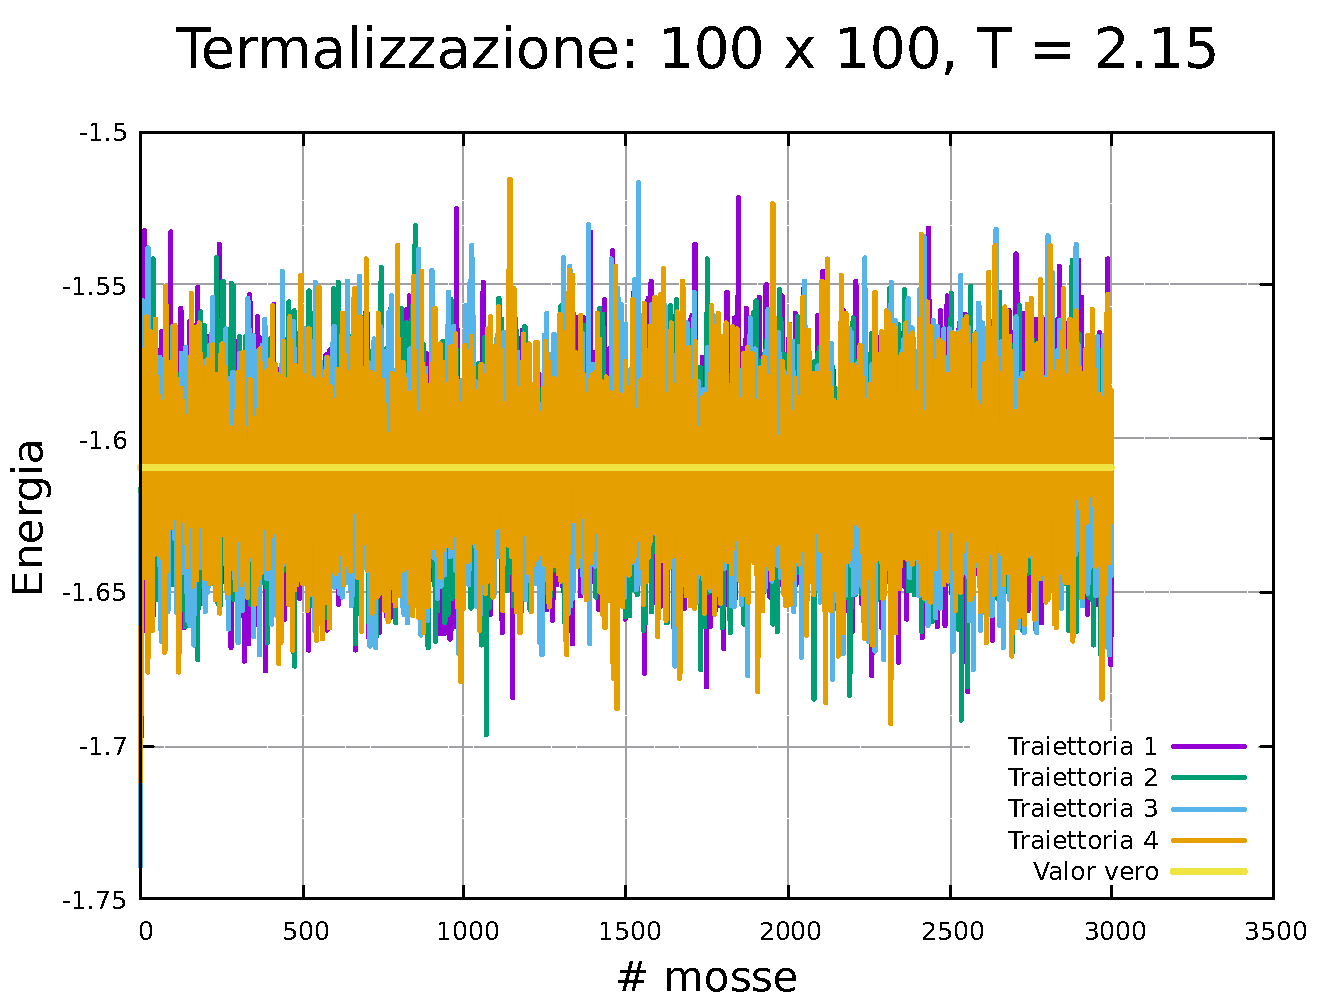
\includegraphics[page=1, width=\textwidth]{Immagini/simIsing2D/wolff/term/term_100_2.15.pdf}
      \caption{$T\,=\,1.5$}
    \end{minipage}
    \vskip\baselineskip 

    \begin{minipage}{0.45\textwidth}  
        \centering
        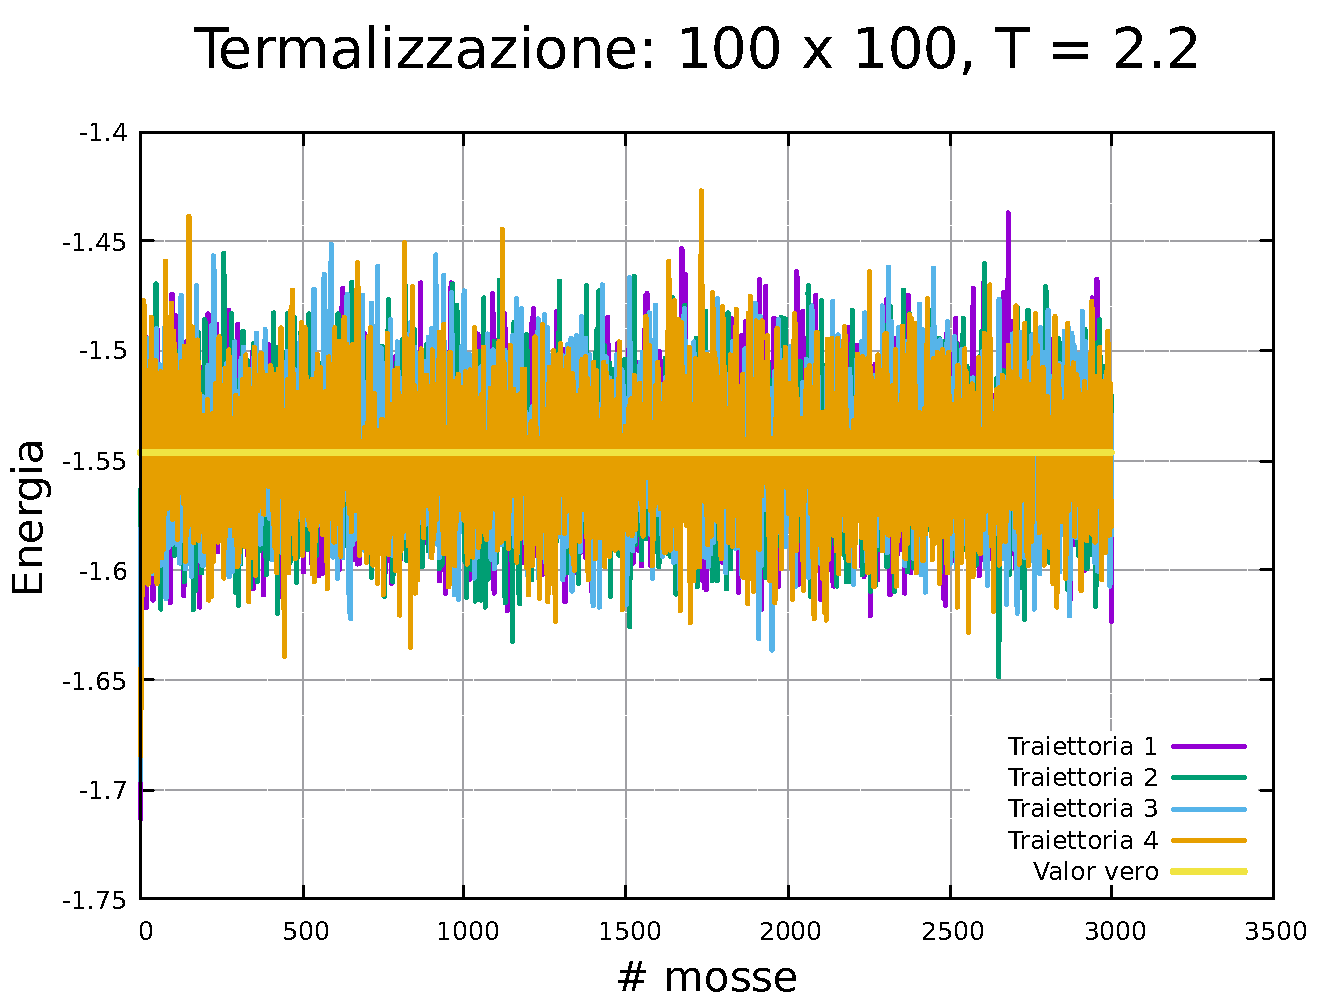
\includegraphics[page=1, width=\textwidth]{Immagini/simIsing2D/wolff/term/term_100_2.2.pdf}
        \caption{$T\,=\,2.0$}
      \end{minipage}\hfill
      \begin{minipage}{0.45\textwidth}  
        \centering
        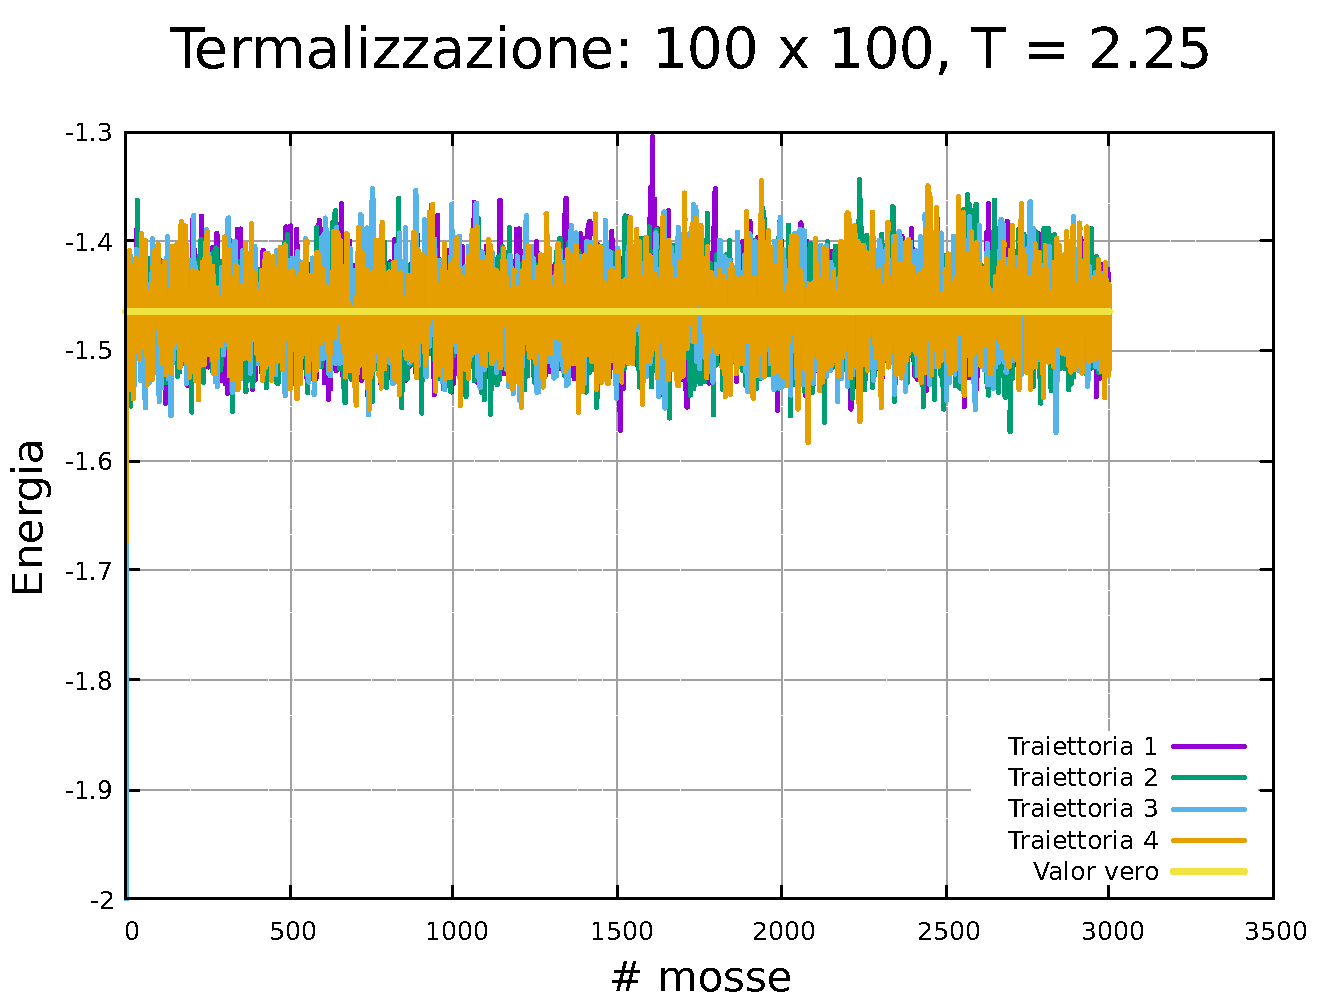
\includegraphics[page=1, width=\textwidth]{Immagini/simIsing2D/wolff/term/term_100_2.25.pdf}
        \caption{$T\,=\,2.5$}
      \end{minipage}
    \vskip\baselineskip 
  
    \begin{minipage}{0.45\textwidth}  
      \centering
      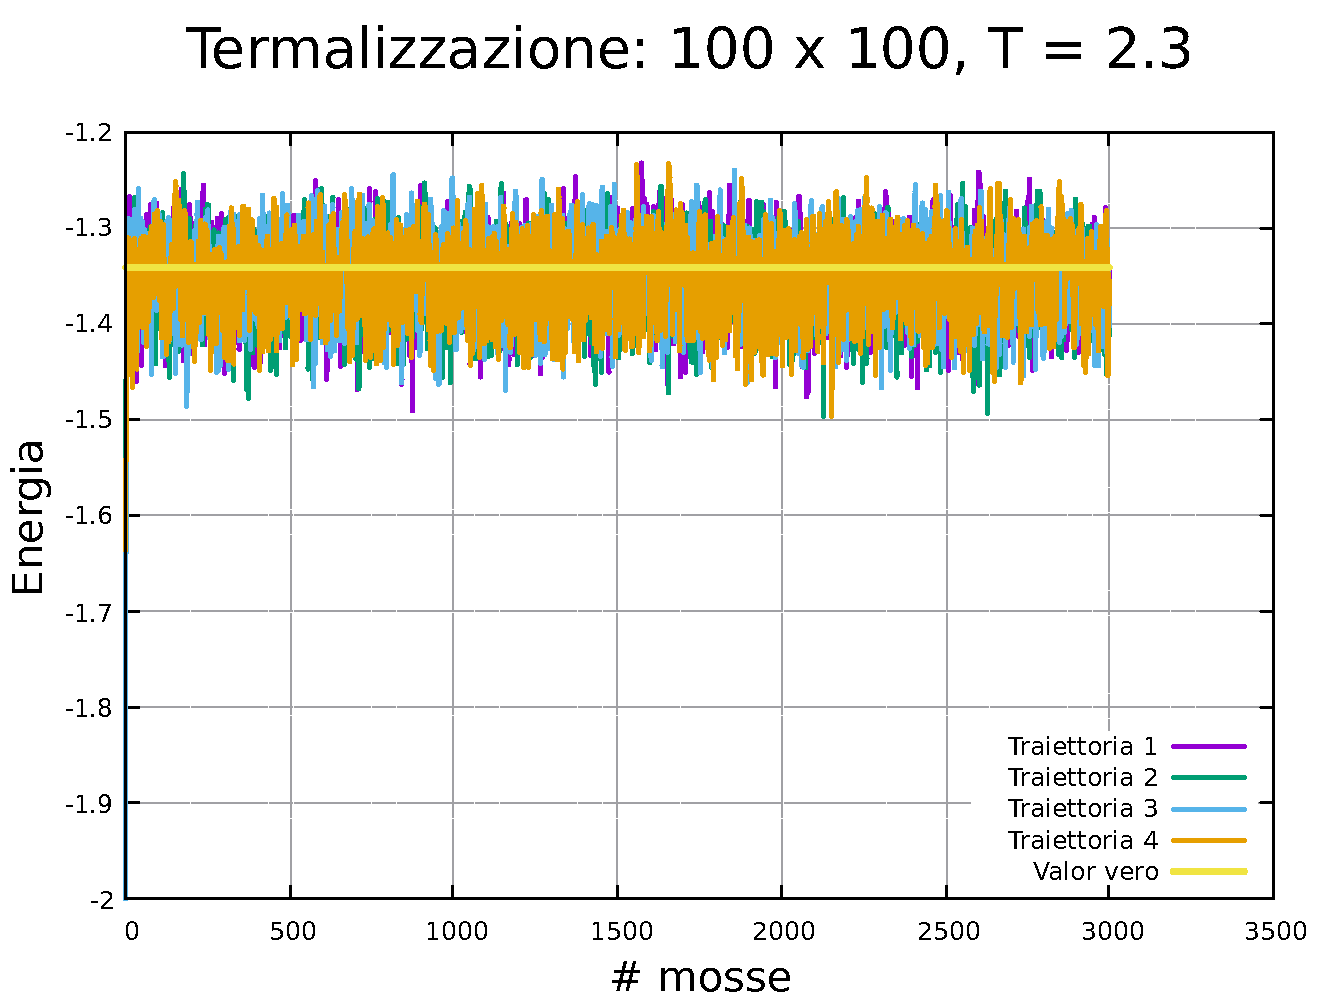
\includegraphics[page=1, width=\textwidth]{Immagini/simIsing2D/wolff/term/term_100_2.3.pdf}
      \caption{$T\,=\,3.0$}
    \end{minipage}\hfill
    \begin{minipage}{0.45\textwidth}  
      \centering
      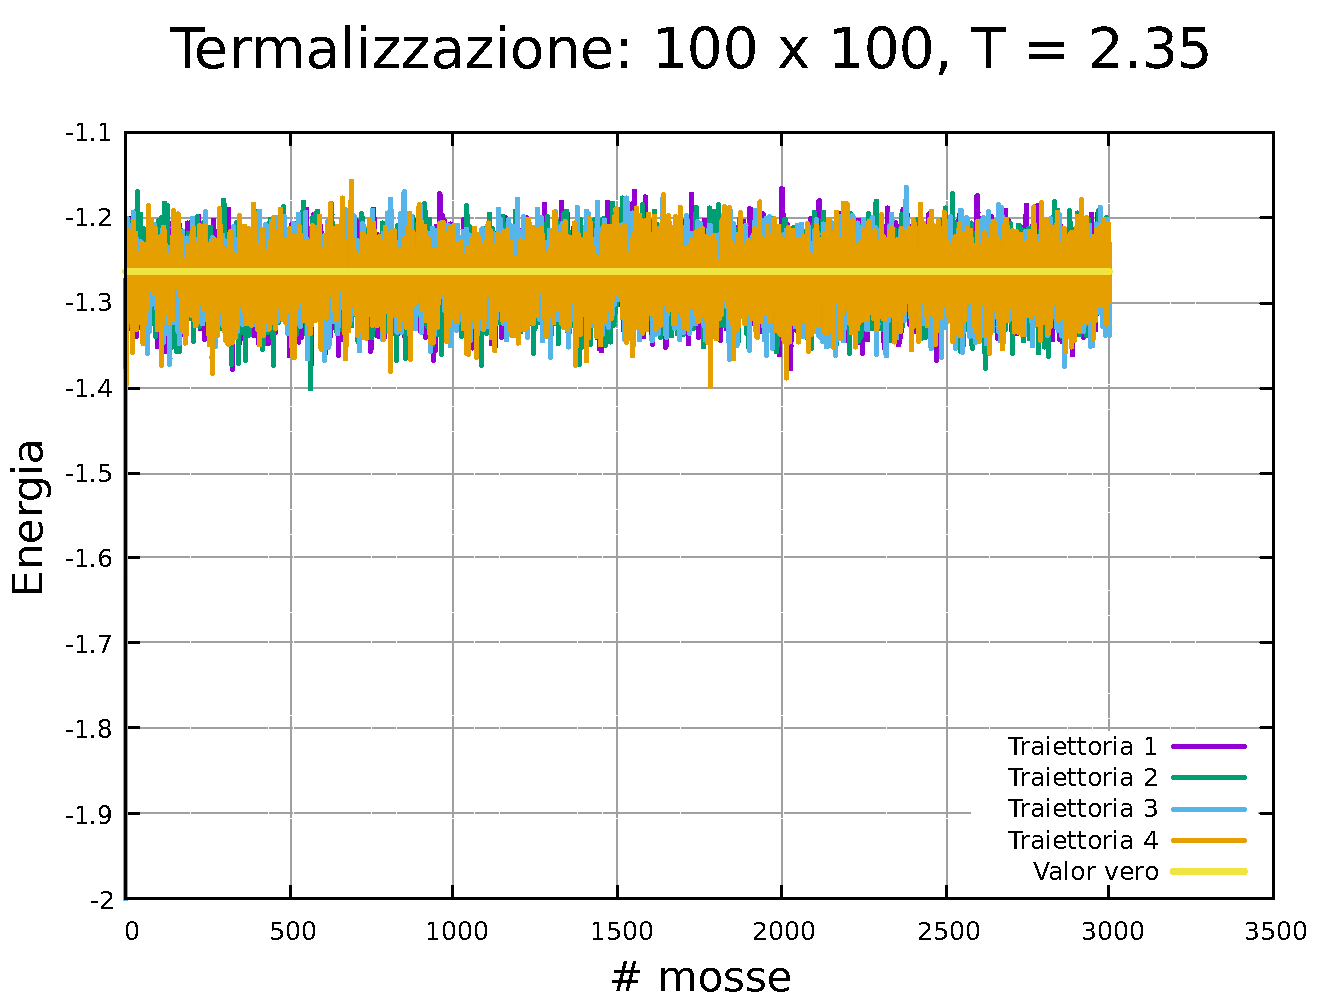
\includegraphics[page=1, width=\textwidth]{Immagini/simIsing2D/wolff/term/term_100_2.35.pdf}
      \caption{$T\,=\,3.5$}
    \end{minipage}
    \caption{Studio della termalizzazione di un modello di Ising 2D: $100 \times 100$, h = 0.0.}
\end{figure}

\vspace*{\fill}



\vspace*{\fill}

\begin{figure}[H]
    \centering
    \begin{minipage}{0.45\textwidth}  
      \centering
      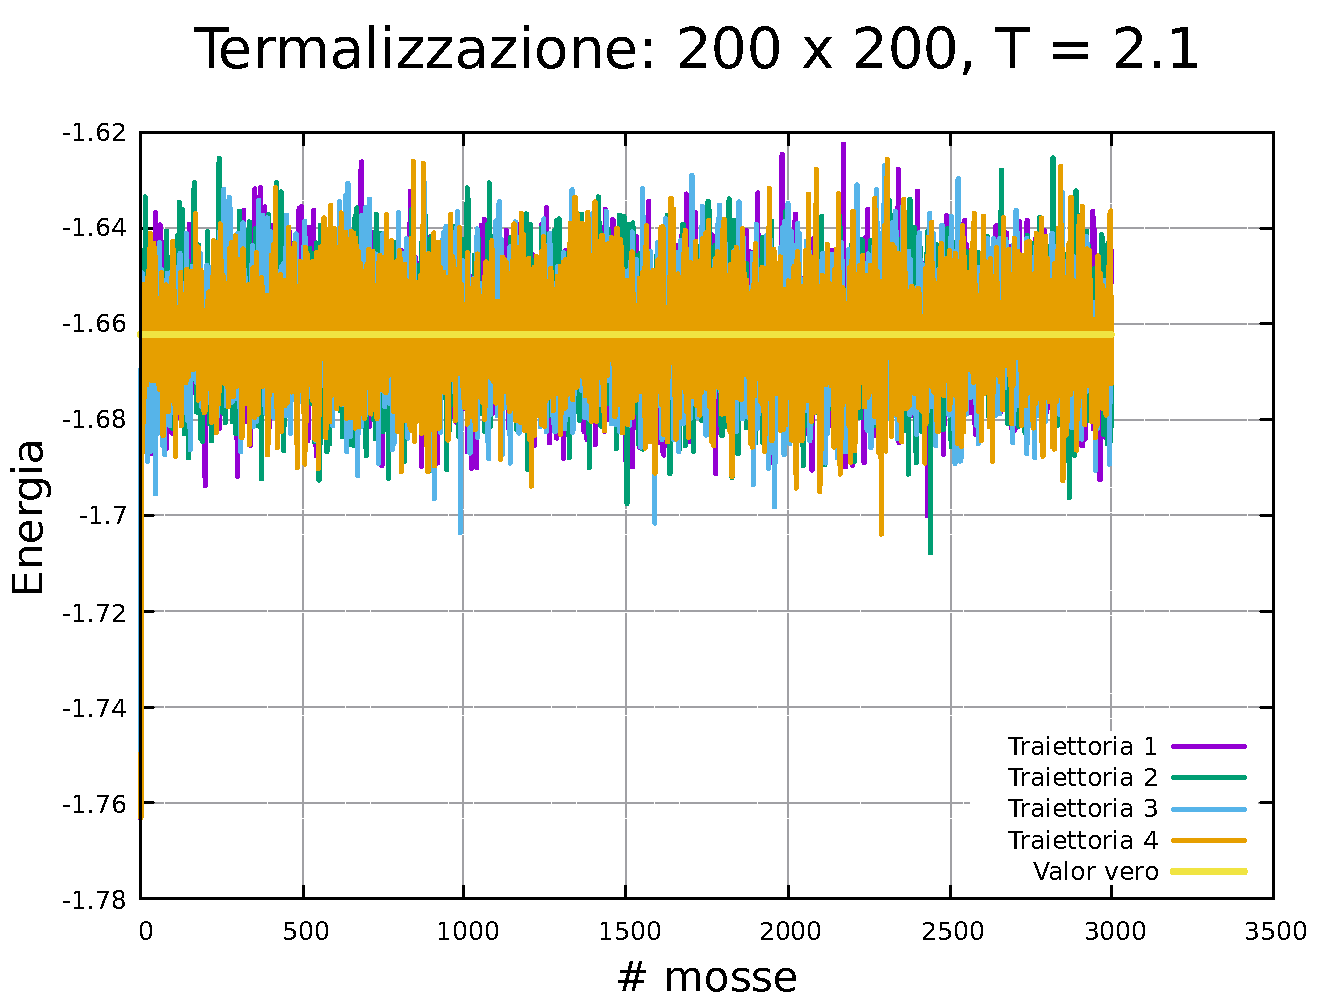
\includegraphics[page=1, width=\textwidth]{Immagini/simIsing2D/wolff/term/term_200_2.1.pdf}
      \caption{$T\,=\,1.0$}
    \end{minipage}\hfill
    \begin{minipage}{0.45\textwidth}  
      \centering
      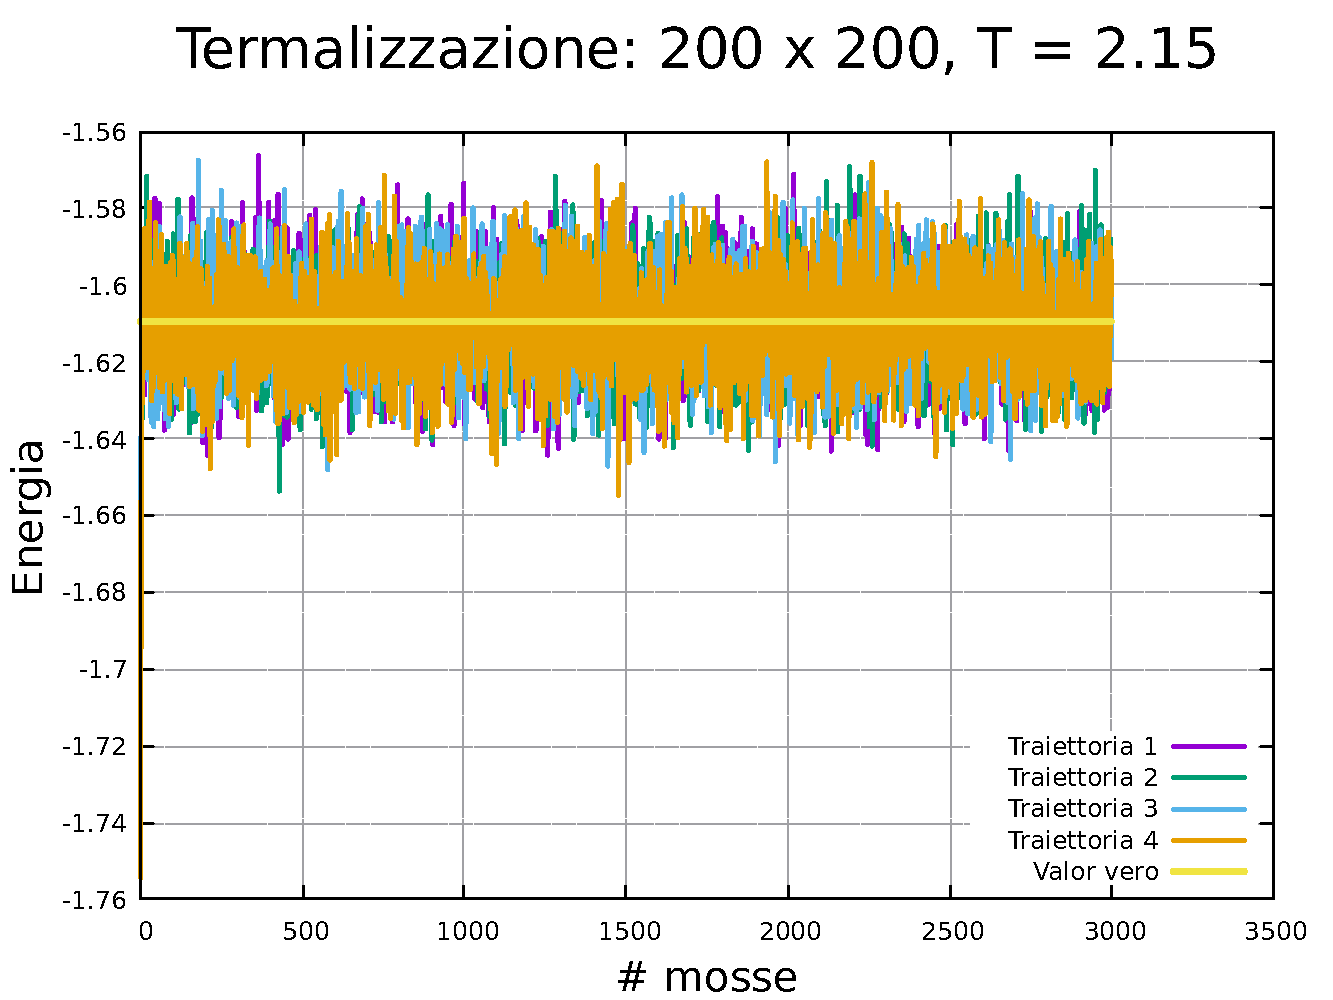
\includegraphics[page=1, width=\textwidth]{Immagini/simIsing2D/wolff/term/term_200_2.15.pdf}
      \caption{$T\,=\,1.5$}
    \end{minipage}
    \vskip\baselineskip 
  
    \begin{minipage}{0.45\textwidth}  
      \centering
      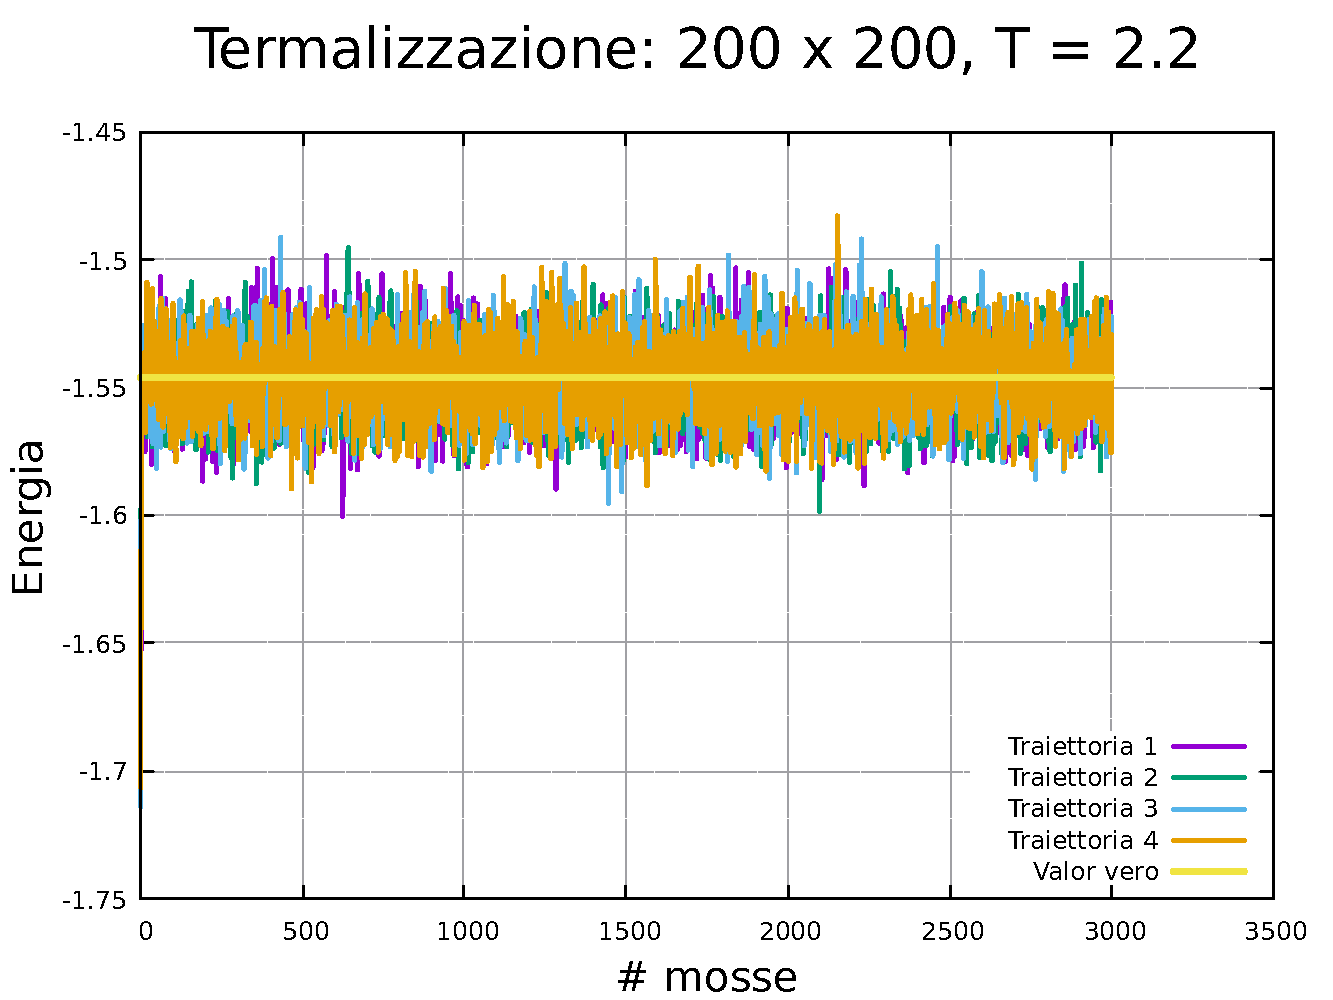
\includegraphics[page=1, width=\textwidth]{Immagini/simIsing2D/wolff/term/term_200_2.2.pdf}
      \caption{$T\,=\,2.0$}
    \end{minipage}\hfill
    \begin{minipage}{0.45\textwidth}  
      \centering
      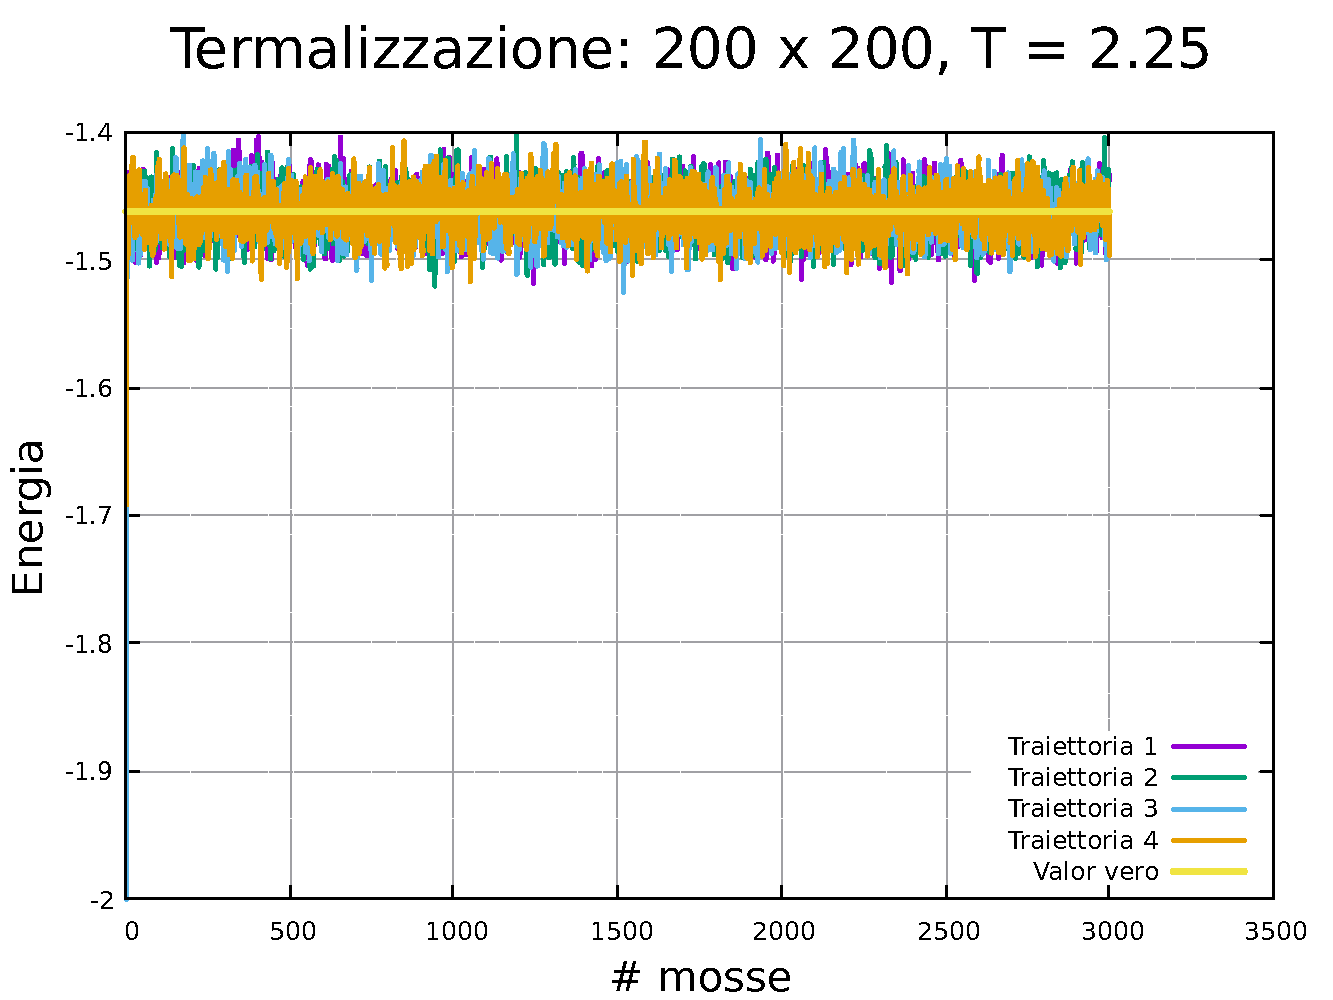
\includegraphics[page=1, width=\textwidth]{Immagini/simIsing2D/wolff/term/term_200_2.25.pdf}
      \caption{$T\,=\,2.5$}
    \end{minipage}
    \vskip\baselineskip 

    \begin{minipage}{0.45\textwidth}  
        \centering
        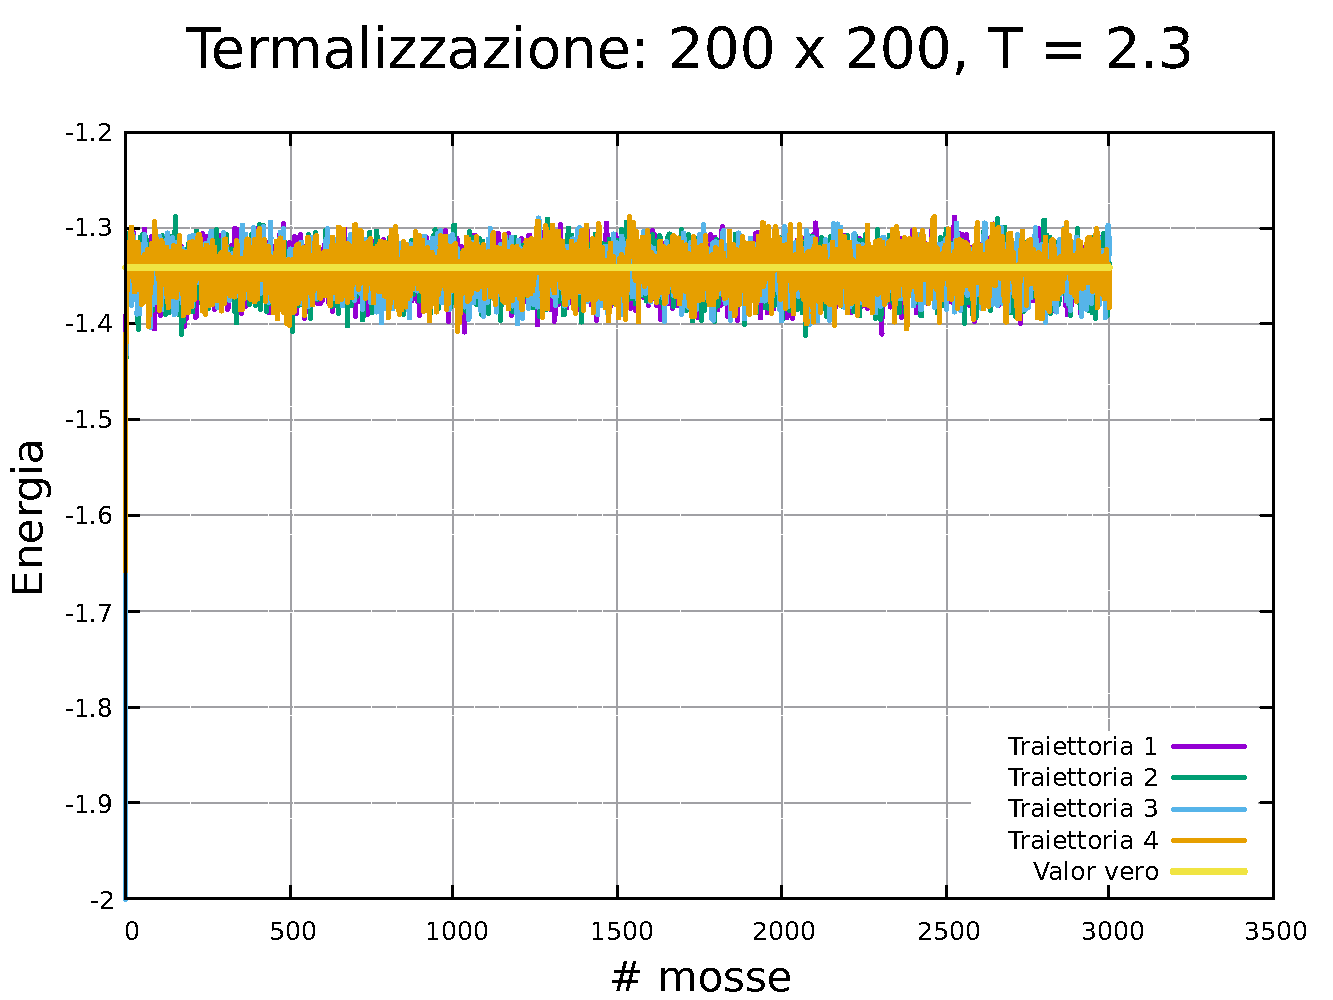
\includegraphics[page=1, width=\textwidth]{Immagini/simIsing2D/wolff/term/term_200_2.3.pdf}
        \caption{$T\,=\,3.0$}
      \end{minipage}\hfill
      \begin{minipage}{0.45\textwidth}  
        \centering
        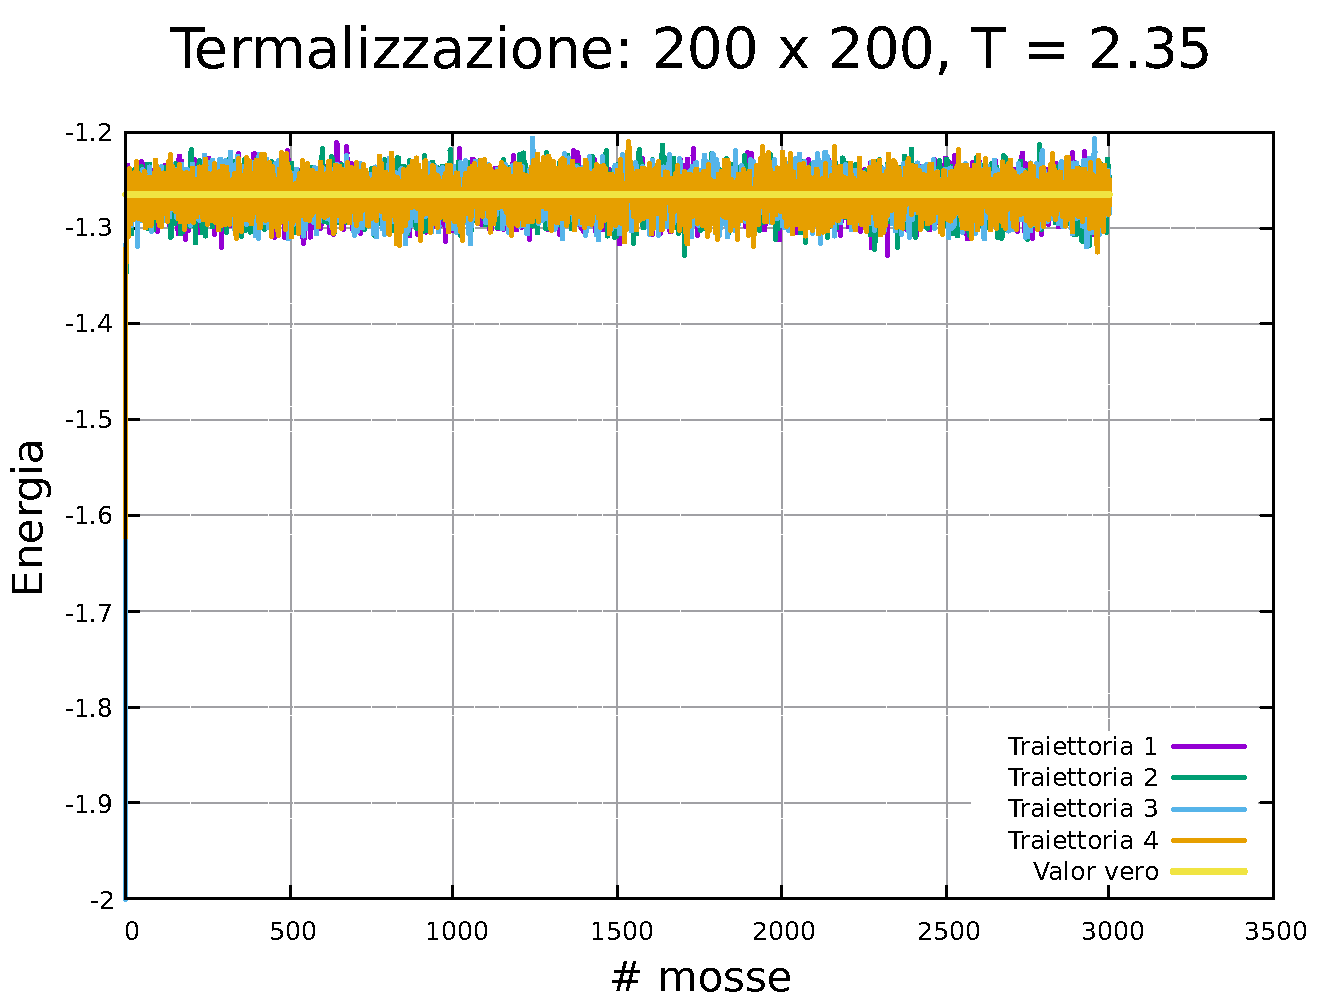
\includegraphics[page=1, width=\textwidth]{Immagini/simIsing2D/wolff/term/term_200_2.35.pdf}
        \caption{$T\,=\,3.5$}
    \end{minipage}

    \caption{Studio della termalizzazione di un modello di Ising 2D: $200 \times 200$, h = 0.0.}
\end{figure}

\vspace*{\fill}



\vspace*{\fill}

\begin{figure}[H]
    \centering
    \begin{minipage}{0.45\textwidth}  
      \centering
      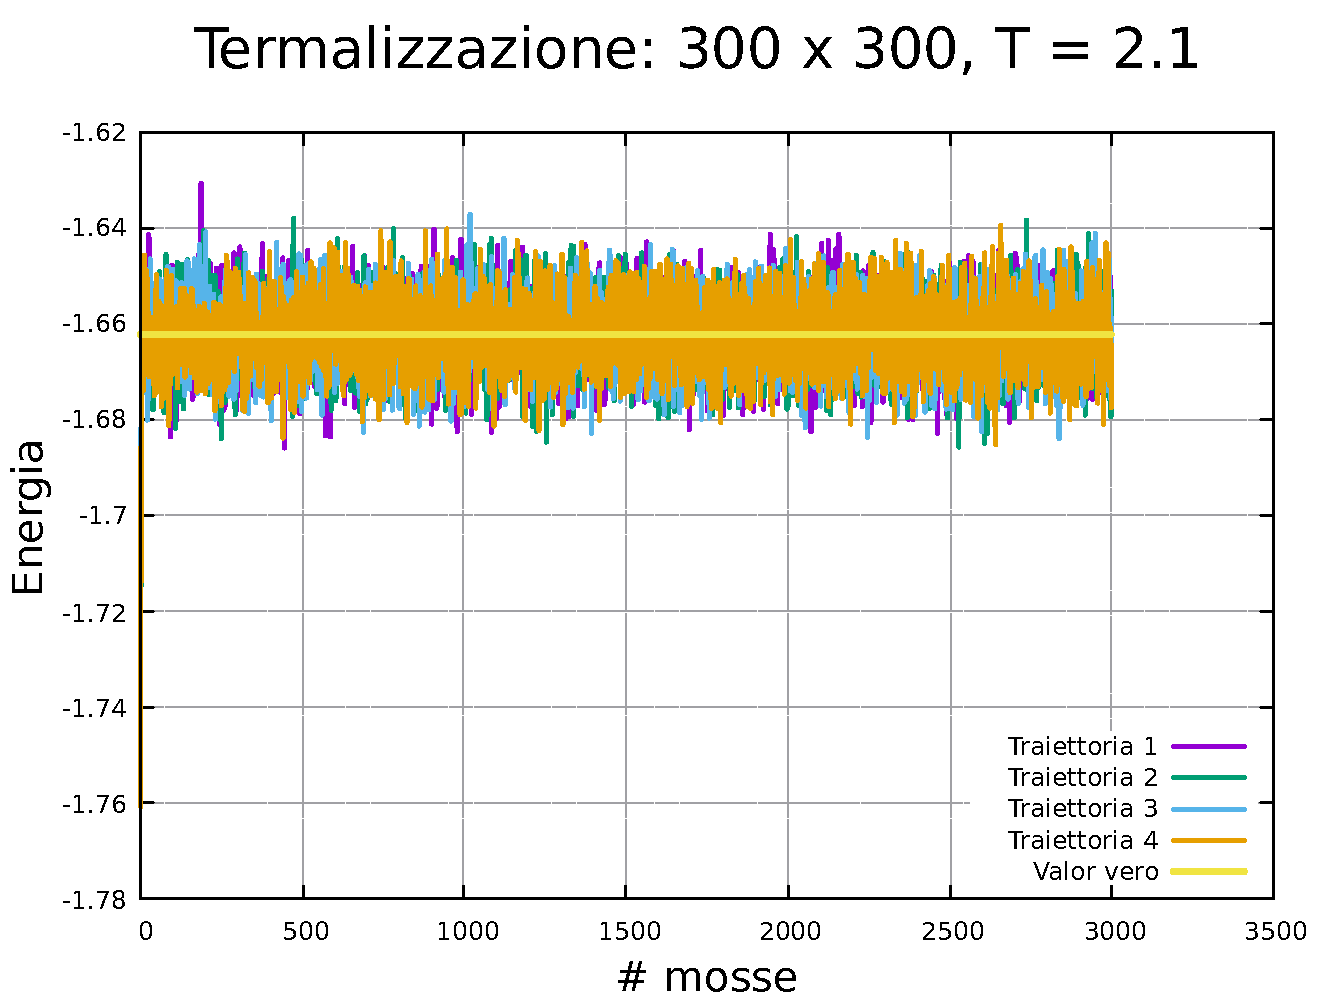
\includegraphics[page=1, width=\textwidth]{Immagini/simIsing2D/wolff/term/term_300_2.1.pdf}
      \caption{$T\,=\,1.0$}
    \end{minipage}\hfill
    \begin{minipage}{0.45\textwidth}  
      \centering
      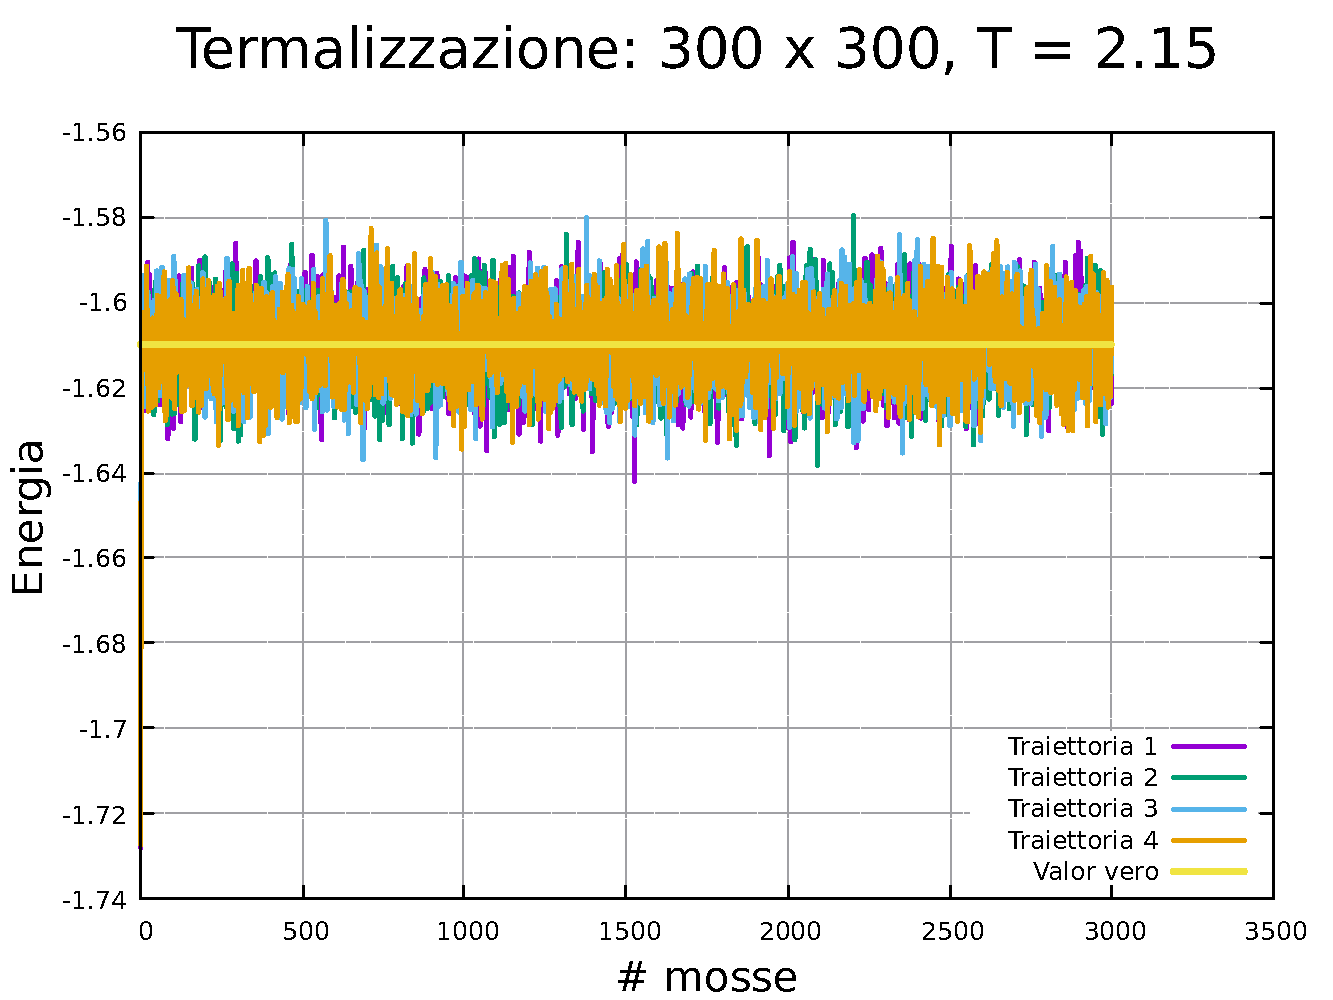
\includegraphics[page=1, width=\textwidth]{Immagini/simIsing2D/wolff/term/term_300_2.15.pdf}
      \caption{$T\,=\,1.5$}
    \end{minipage}
    \vskip\baselineskip 

    \begin{minipage}{0.45\textwidth}  
        \centering
        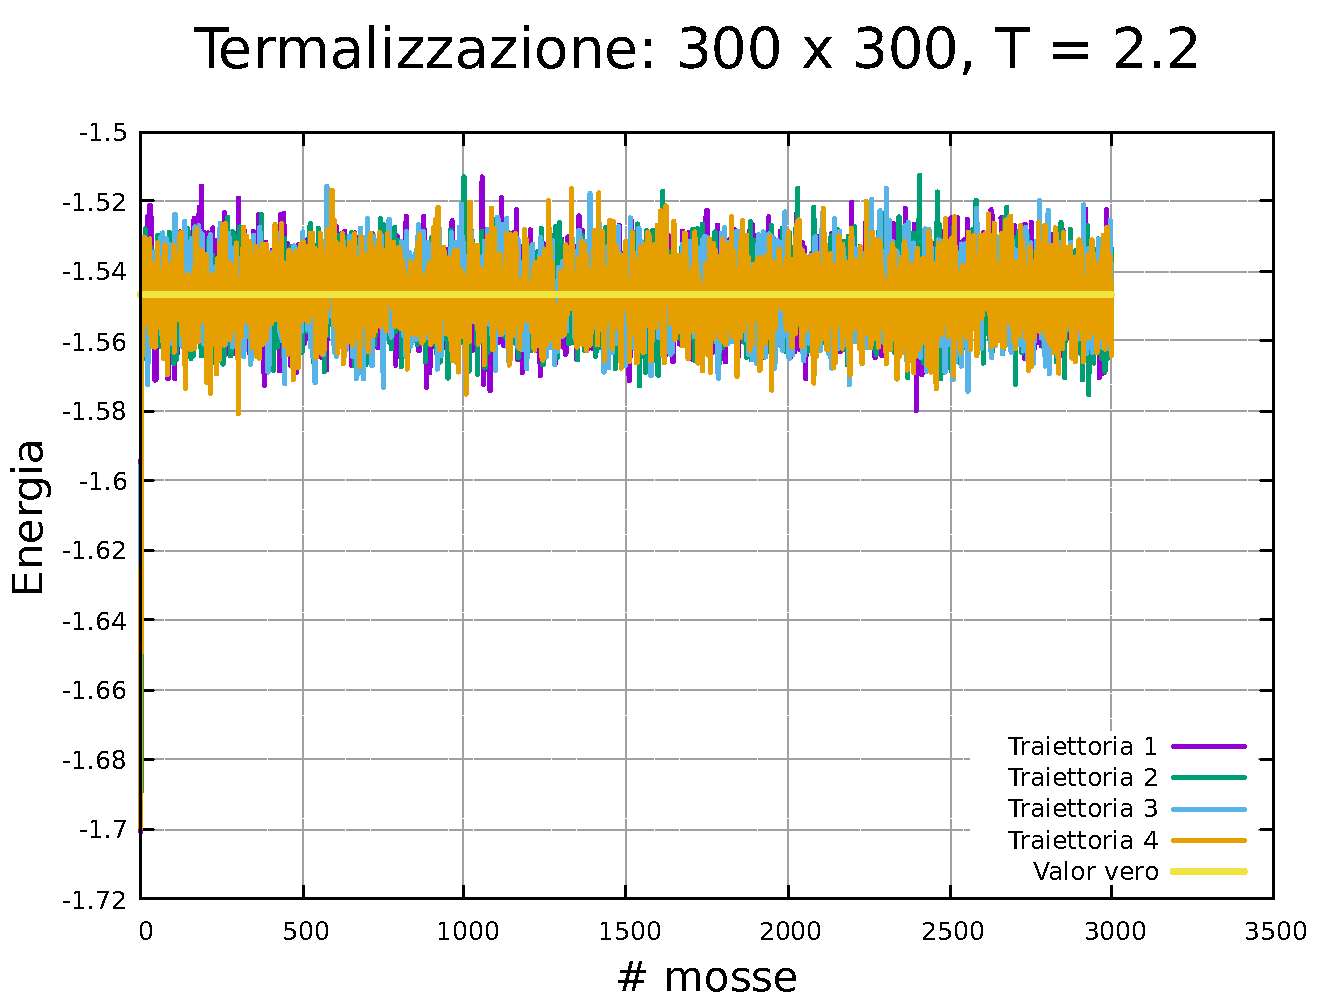
\includegraphics[page=1, width=\textwidth]{Immagini/simIsing2D/wolff/term/term_300_2.2.pdf}
        \caption{$T\,=\,2.0$}
      \end{minipage}\hfill
      \begin{minipage}{0.45\textwidth}  
        \centering
        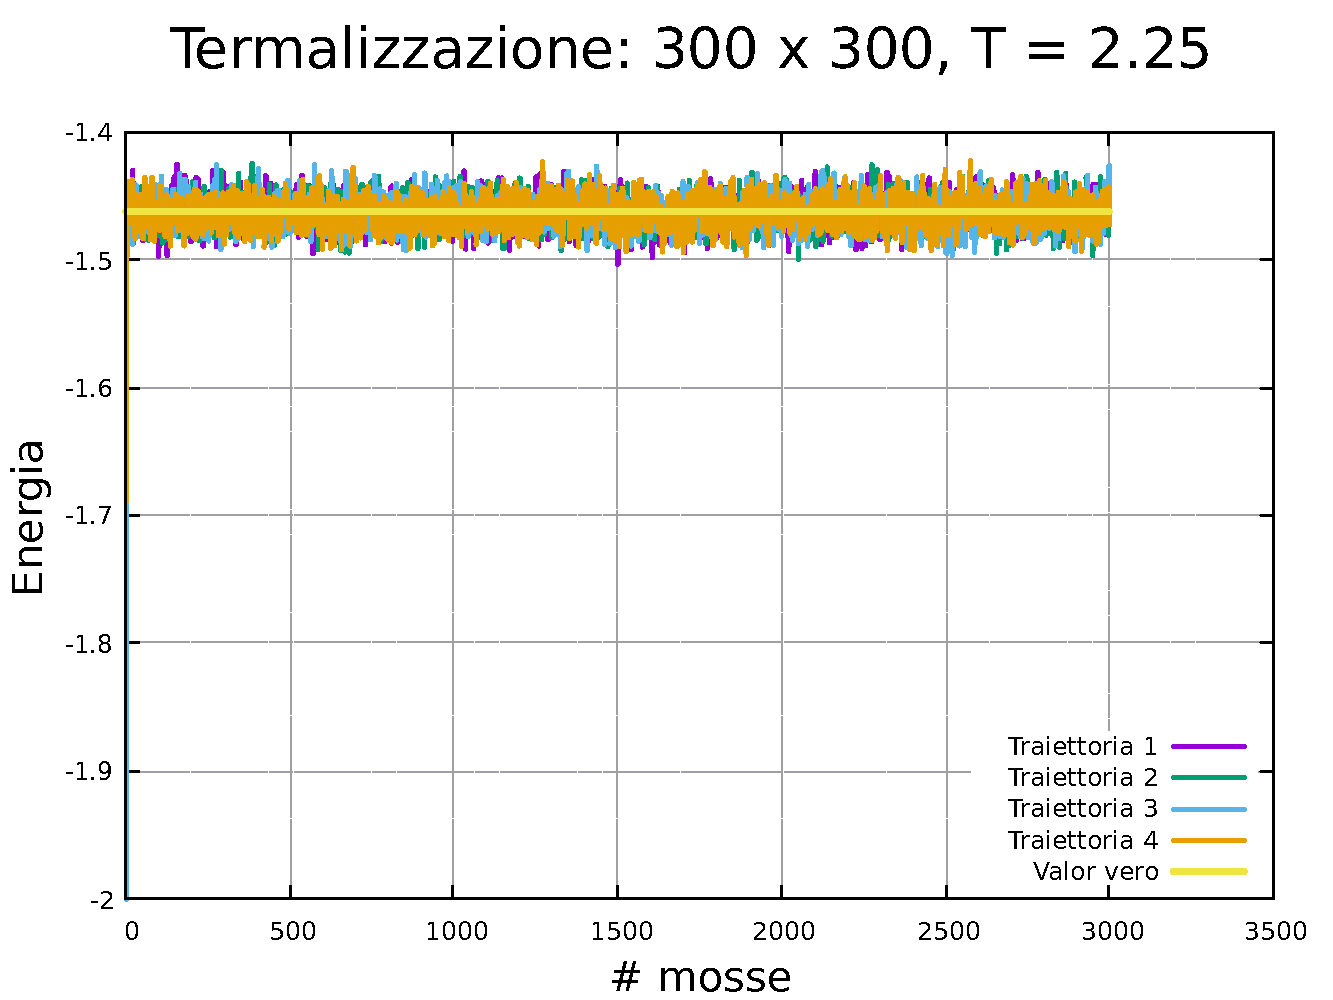
\includegraphics[page=1, width=\textwidth]{Immagini/simIsing2D/wolff/term/term_300_2.25.pdf}
        \caption{$T\,=\,2.5$}
      \end{minipage}
    \vskip\baselineskip 
  
    \begin{minipage}{0.45\textwidth}  
      \centering
      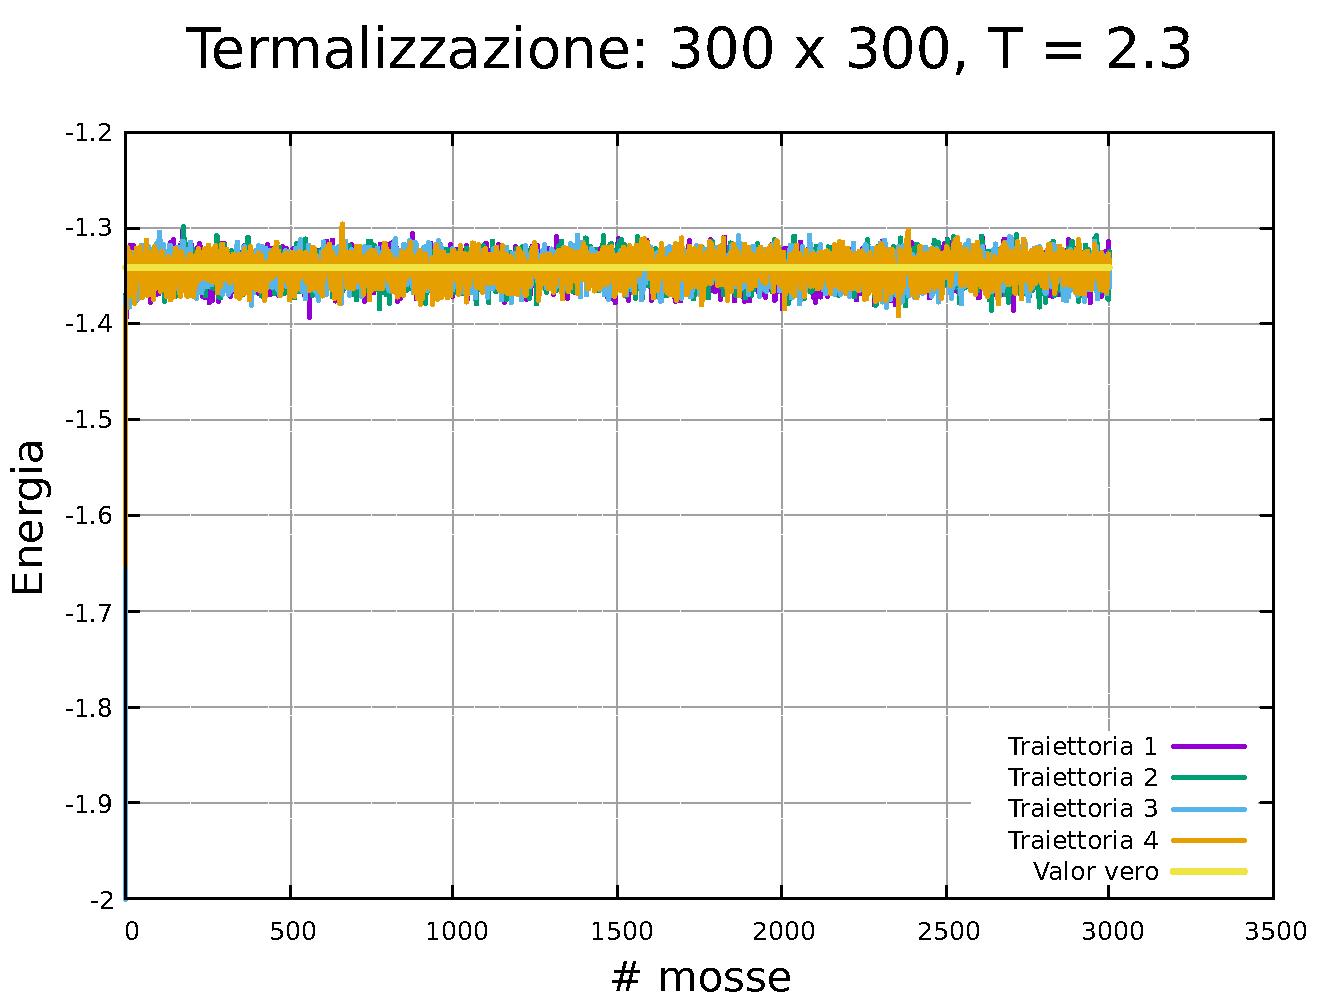
\includegraphics[page=1, width=\textwidth]{Immagini/simIsing2D/wolff/term/term_300_2.3.pdf}
      \caption{$T\,=\,3.0$}
    \end{minipage}\hfill
    \begin{minipage}{0.45\textwidth}  
      \centering
      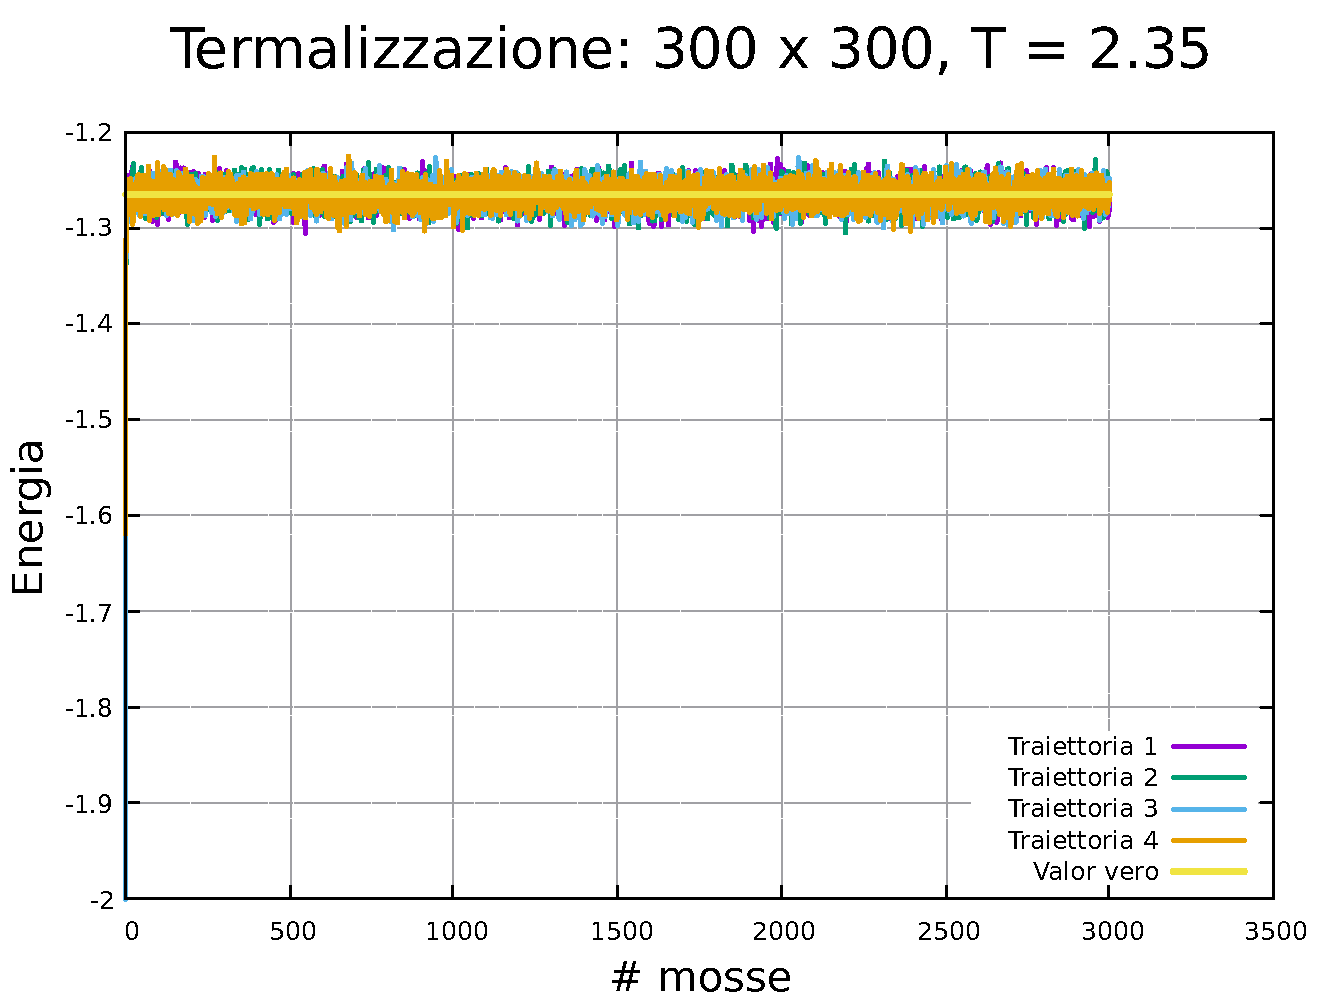
\includegraphics[page=1, width=\textwidth]{Immagini/simIsing2D/wolff/term/term_300_2.35.pdf}
      \caption{$T\,=\,3.5$}
    \end{minipage}
    \caption{Studio della termalizzazione di un modello di Ising 2D: $300 \times 300$, h = 0.0.}
\end{figure}

\vspace*{\fill}



\vspace*{\fill}

\begin{figure}[H]
    \centering
    \begin{minipage}{0.45\textwidth}  
      \centering
      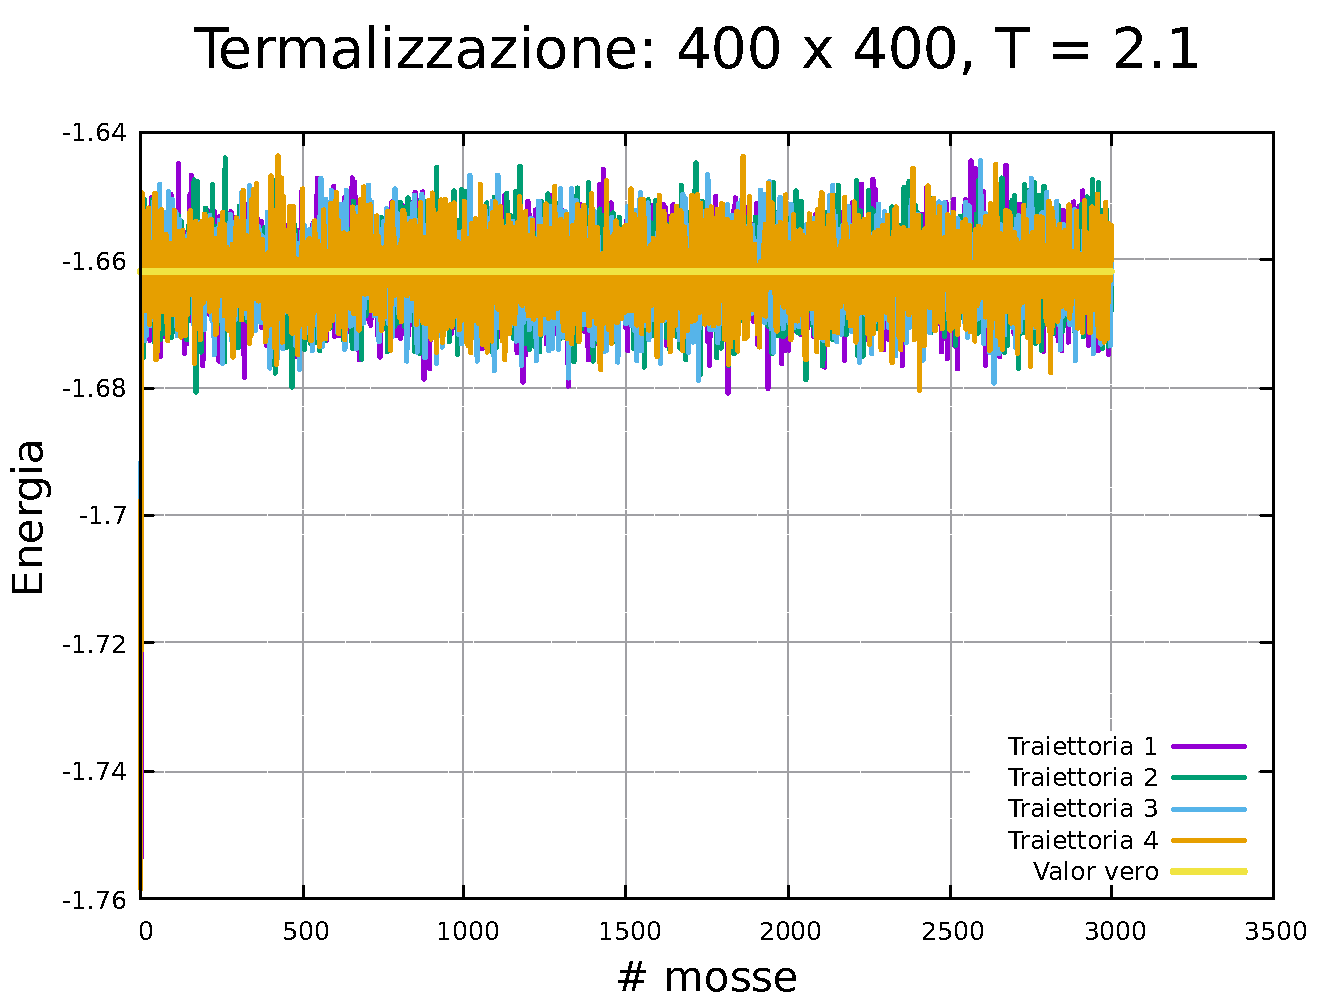
\includegraphics[page=1, width=\textwidth]{Immagini/simIsing2D/wolff/term/term_400_2.1.pdf}
      \caption{$T\,=\,1.0$}
    \end{minipage}\hfill
    \begin{minipage}{0.45\textwidth}  
      \centering
      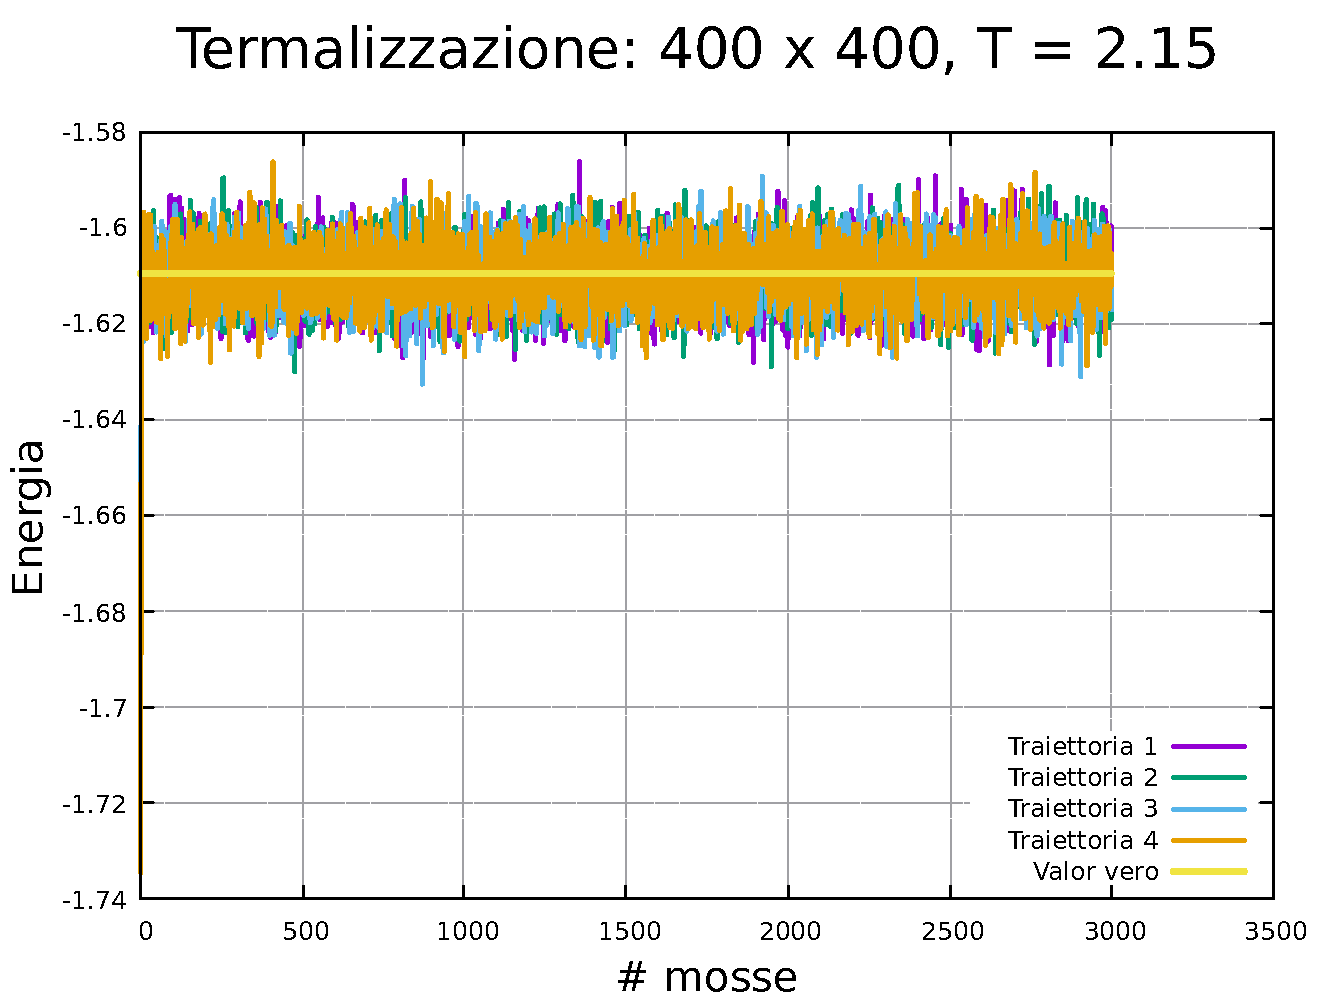
\includegraphics[page=1, width=\textwidth]{Immagini/simIsing2D/wolff/term/term_400_2.15.pdf}
      \caption{$T\,=\,1.5$}
    \end{minipage}
    \vskip\baselineskip 

    \begin{minipage}{0.45\textwidth}  
        \centering
        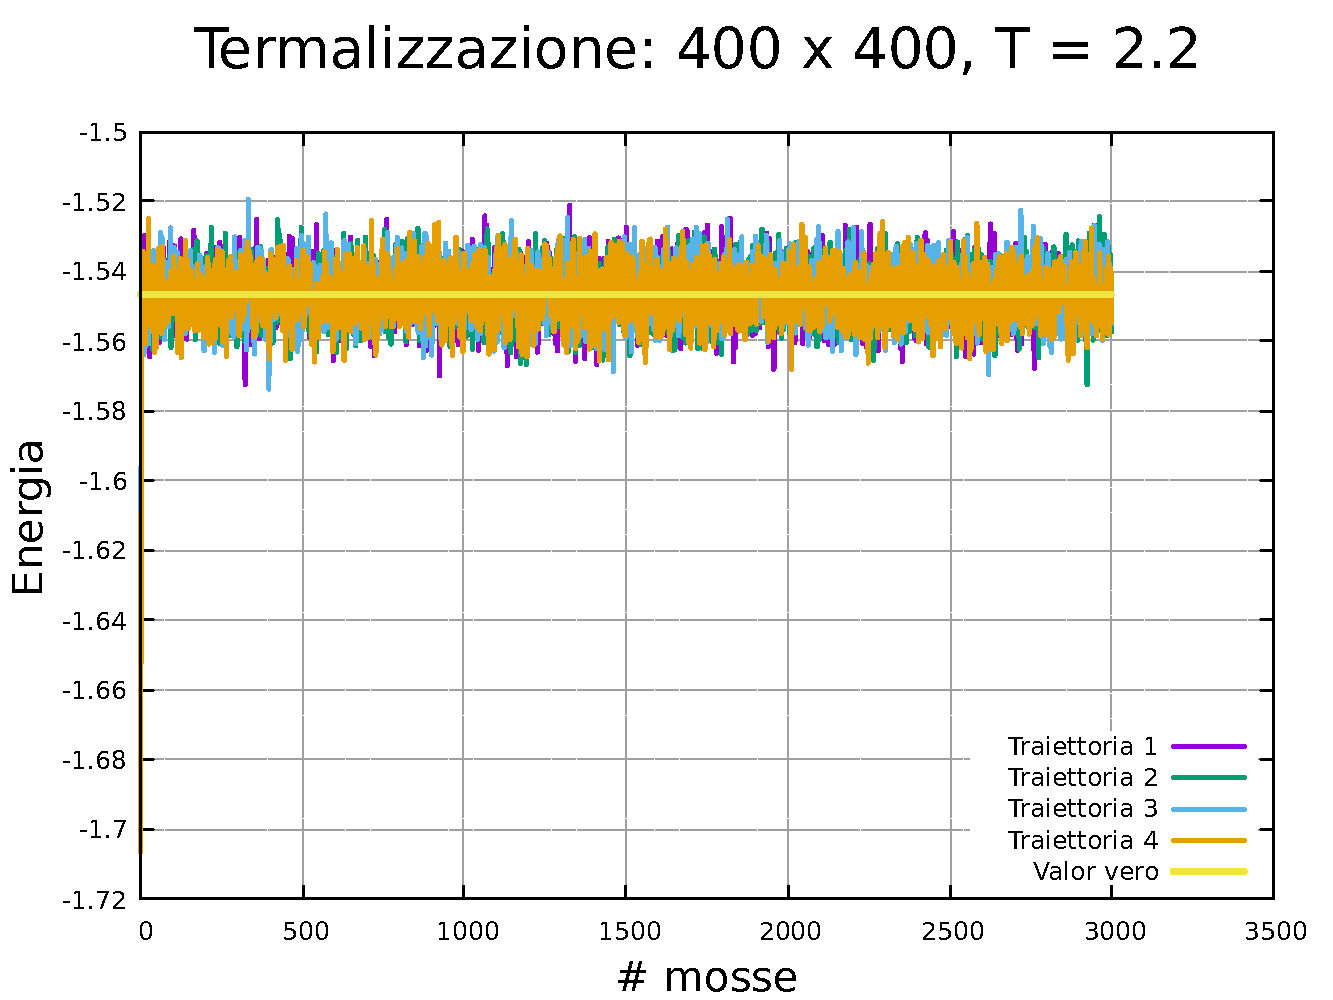
\includegraphics[page=1, width=\textwidth]{Immagini/simIsing2D/wolff/term/term_400_2.2.pdf}
        \caption{$T\,=\,2.0$}
      \end{minipage}\hfill
      \begin{minipage}{0.45\textwidth}  
        \centering
        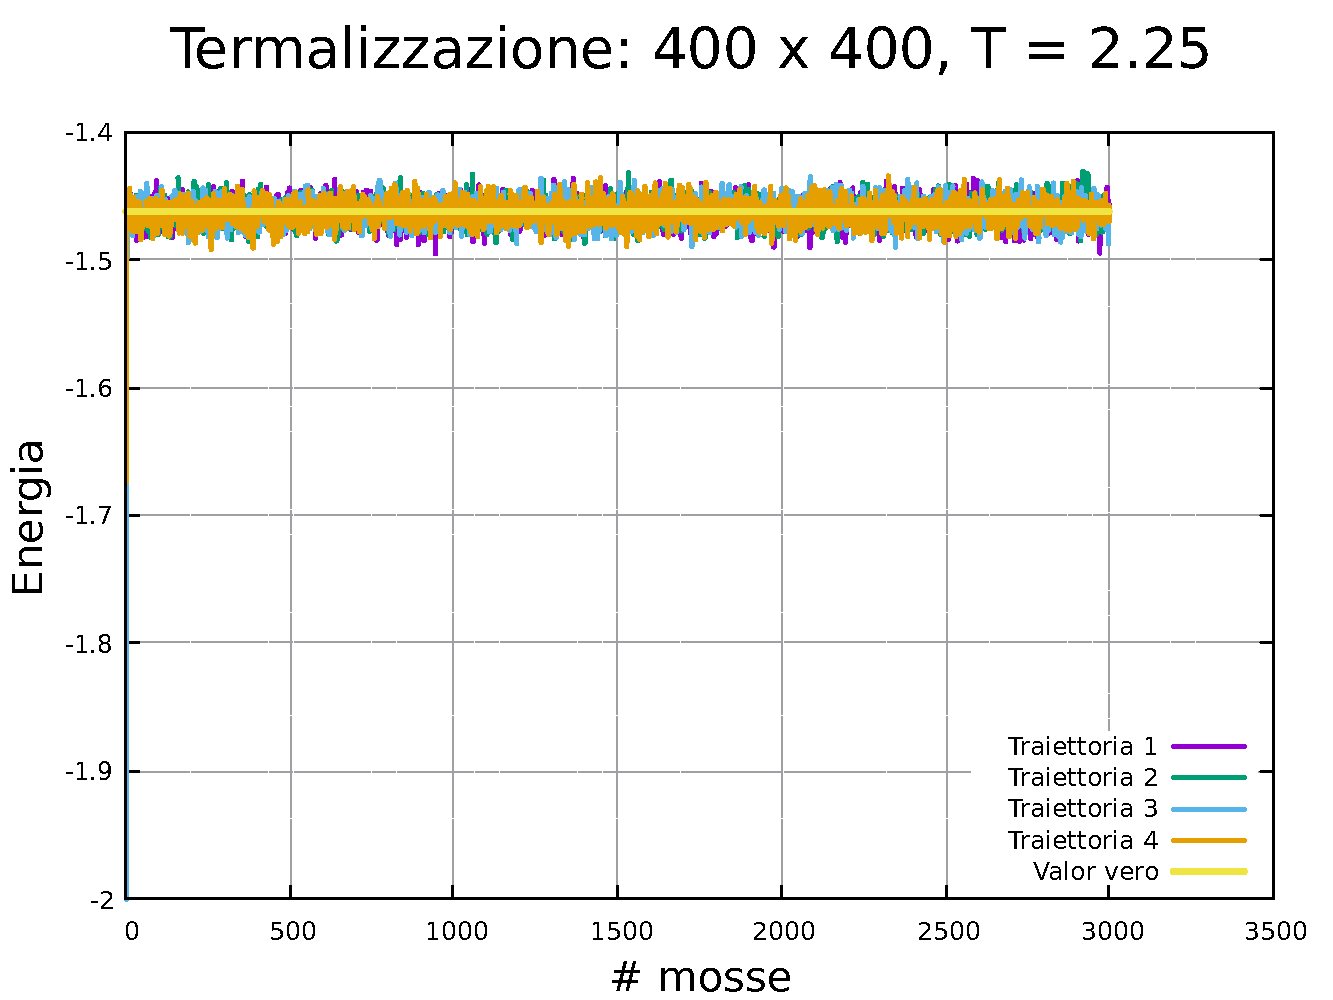
\includegraphics[page=1, width=\textwidth]{Immagini/simIsing2D/wolff/term/term_400_2.25.pdf}
        \caption{$T\,=\,2.5$}
      \end{minipage}
    \vskip\baselineskip 
  
    \begin{minipage}{0.45\textwidth}  
      \centering
      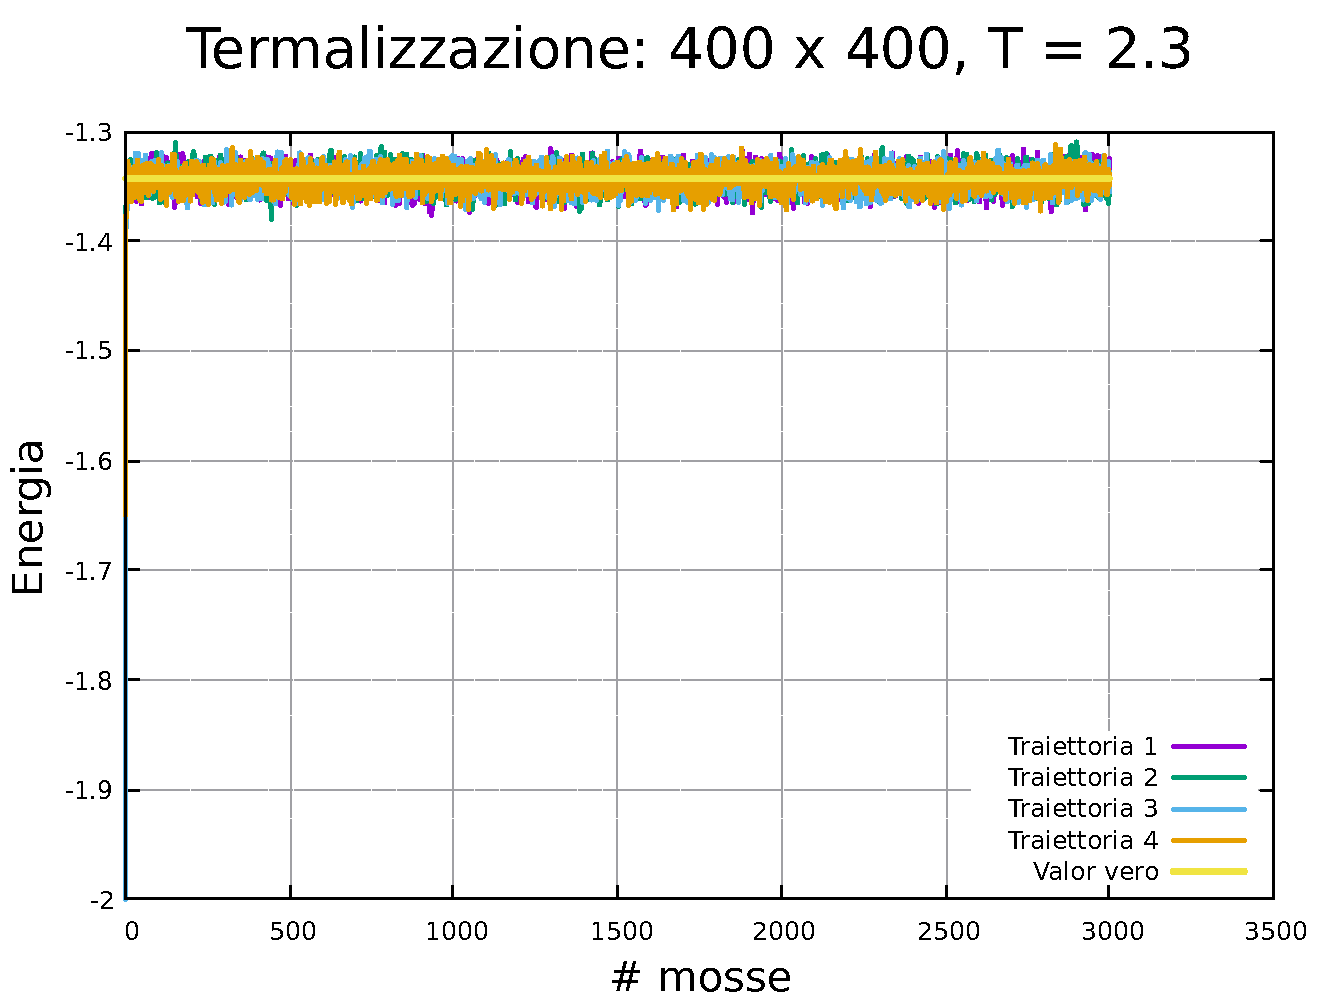
\includegraphics[page=1, width=\textwidth]{Immagini/simIsing2D/wolff/term/term_400_2.3.pdf}
      \caption{$T\,=\,3.0$}
    \end{minipage}\hfill
    \begin{minipage}{0.45\textwidth}  
      \centering
      \includegraphics[page=1, width=\textwidth]{Immagini/simIsing2D/wolff/term/term_400_2.35.pdf}
      \caption{$T\,=\,3.5$}
    \end{minipage}
    \caption{Studio della termalizzazione di un modello di Ising 2D: $400 \times 400$, h = 0.0.}
\end{figure}

\vspace*{\fill}



\vspace*{\fill}

\begin{figure}[H]
    \centering
    \begin{minipage}{0.45\textwidth}  
      \centering
      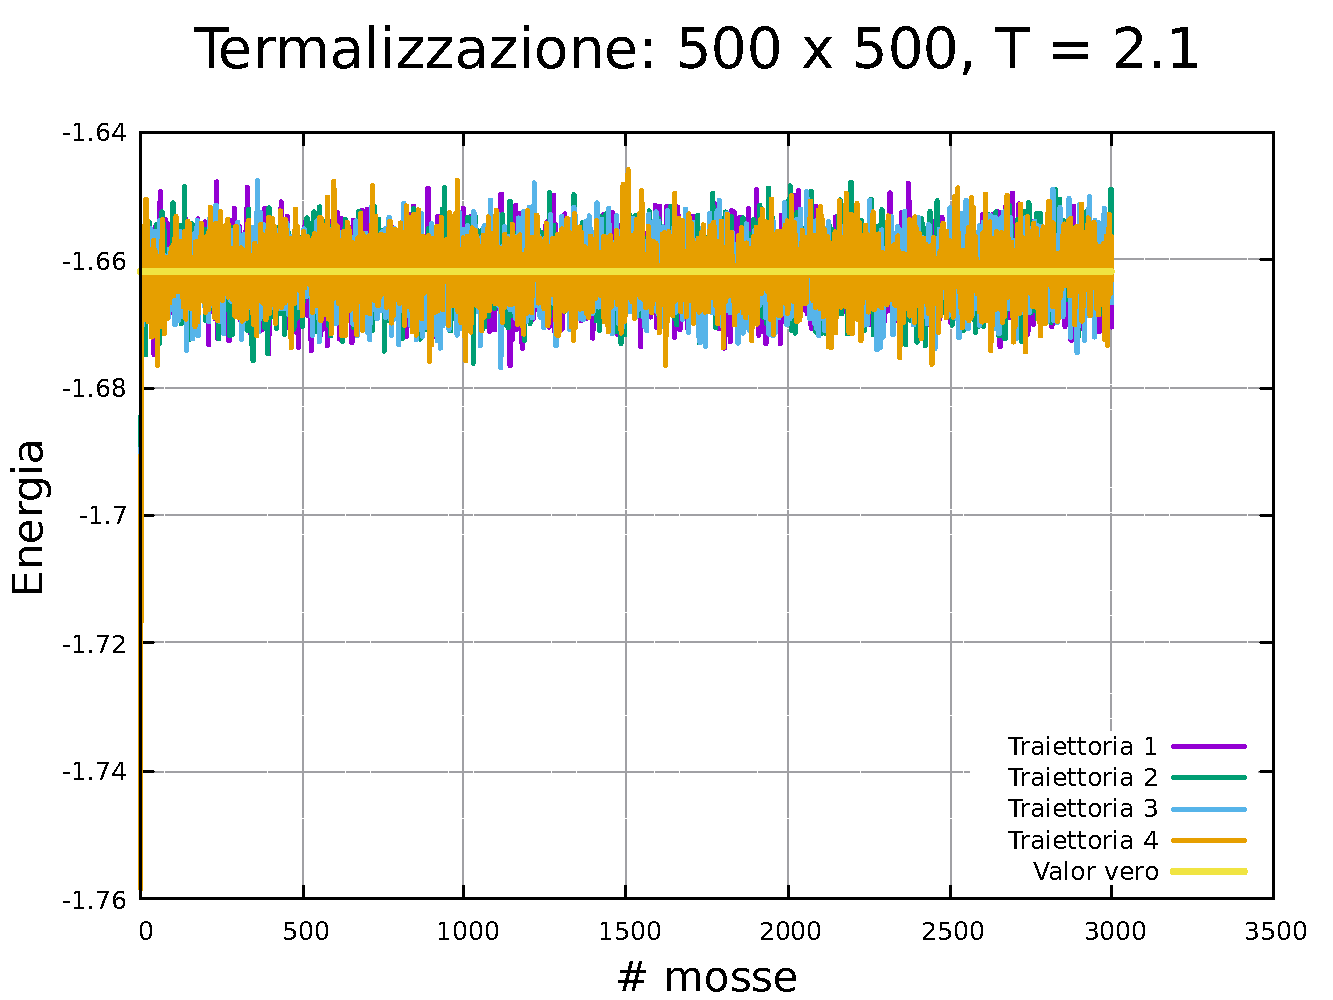
\includegraphics[page=1, width=\textwidth]{Immagini/simIsing2D/wolff/term/term_500_2.1.pdf}
      \caption{$T\,=\,1.0$}
    \end{minipage}\hfill
    \begin{minipage}{0.45\textwidth}  
      \centering
      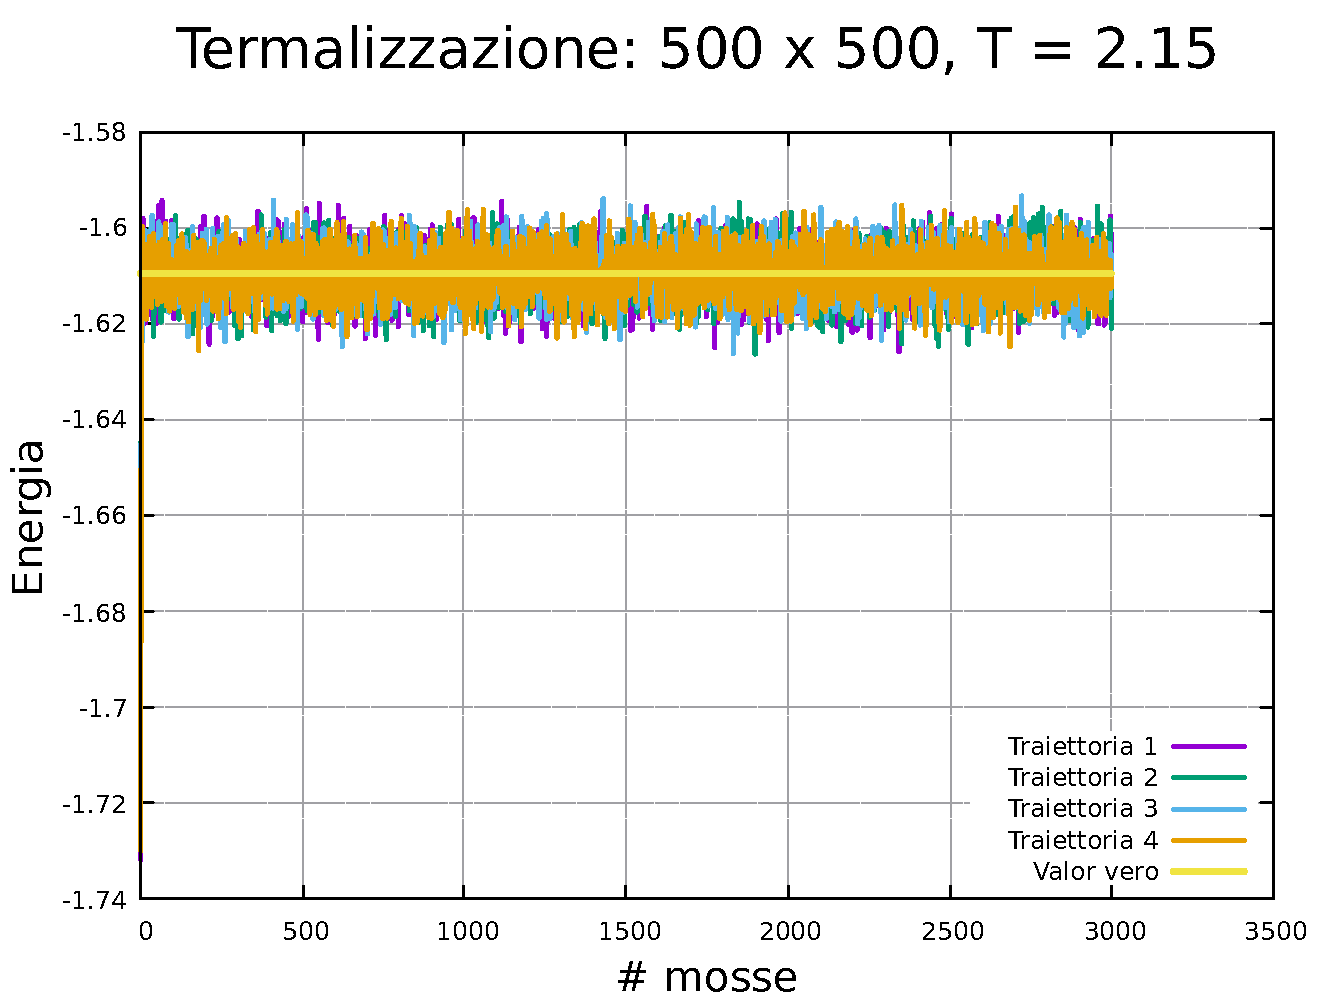
\includegraphics[page=1, width=\textwidth]{Immagini/simIsing2D/wolff/term/term_500_2.15.pdf}
      \caption{$T\,=\,1.5$}
    \end{minipage}
    \vskip\baselineskip 

    \begin{minipage}{0.45\textwidth}  
        \centering
        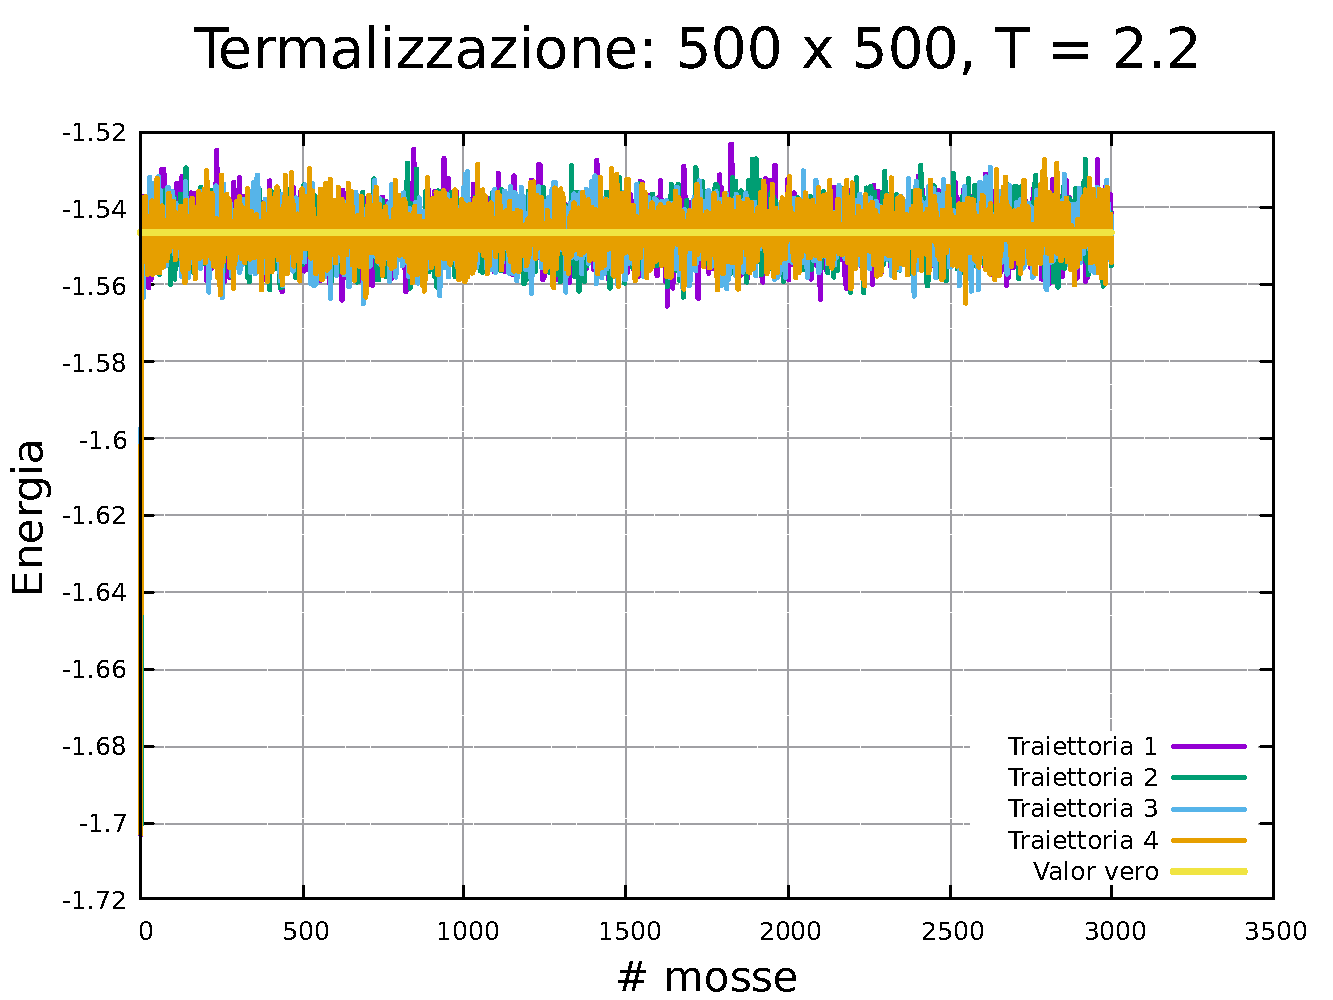
\includegraphics[page=1, width=\textwidth]{Immagini/simIsing2D/wolff/term/term_500_2.2.pdf}
        \caption{$T\,=\,2.0$}
      \end{minipage}\hfill
      \begin{minipage}{0.45\textwidth}  
        \centering
        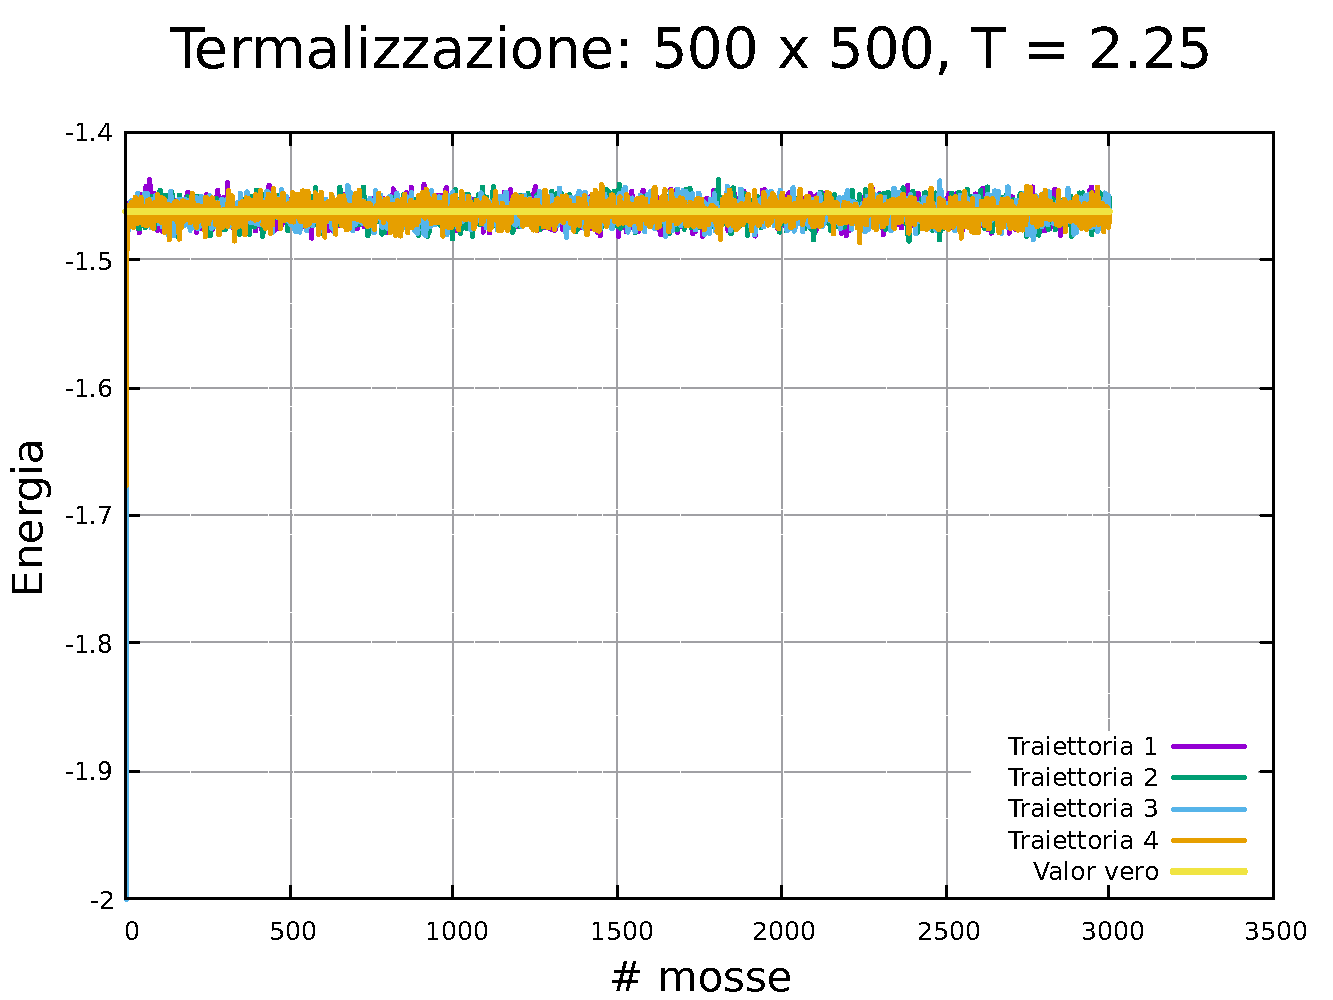
\includegraphics[page=1, width=\textwidth]{Immagini/simIsing2D/wolff/term/term_500_2.25.pdf}
        \caption{$T\,=\,2.5$}
      \end{minipage}
    \vskip\baselineskip 
  
    \begin{minipage}{0.45\textwidth}  
      \centering
      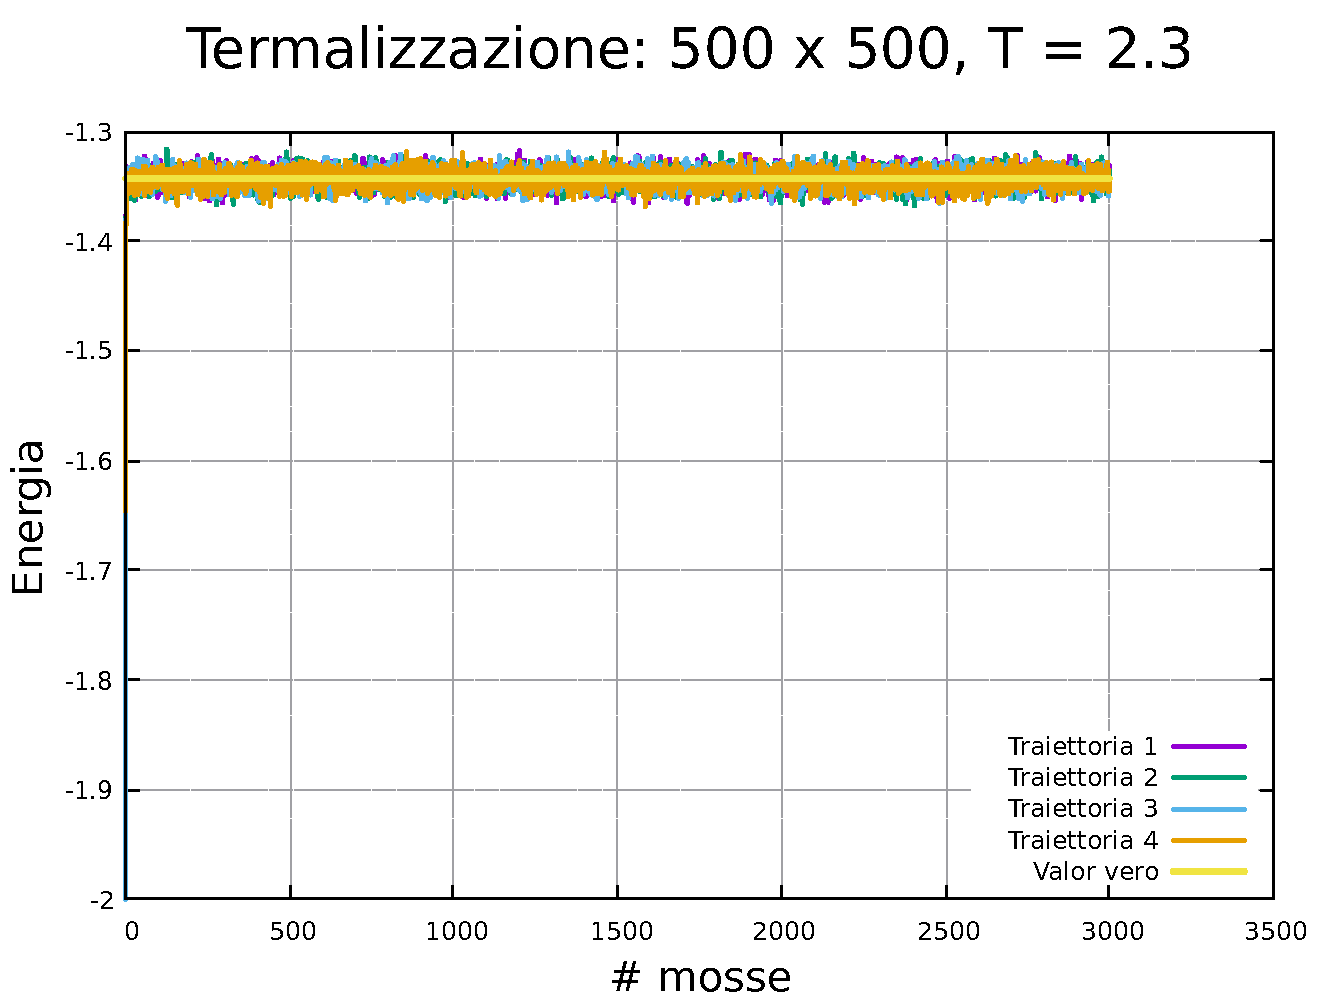
\includegraphics[page=1, width=\textwidth]{Immagini/simIsing2D/wolff/term/term_500_2.3.pdf}
      \caption{$T\,=\,3.0$}
    \end{minipage}\hfill
    \begin{minipage}{0.45\textwidth}  
      \centering
      \includegraphics[page=1, width=\textwidth]{Immagini/simIsing2D/wolff/term/term_500_2.35.pdf}
      \caption{$T\,=\,3.5$}
    \end{minipage}
    \caption{Studio della termalizzazione di un modello di Ising 2D: $500 \times 500$, h = 0.0.}
\end{figure}

\vspace*{\fill}